% Options for packages loaded elsewhere
\PassOptionsToPackage{unicode}{hyperref}
\PassOptionsToPackage{hyphens}{url}
%
\documentclass[
]{article}
\usepackage{lmodern}
\usepackage{amssymb,amsmath}
\usepackage{ifxetex,ifluatex}
\ifnum 0\ifxetex 1\fi\ifluatex 1\fi=0 % if pdftex
  \usepackage[T1]{fontenc}
  \usepackage[utf8]{inputenc}
  \usepackage{textcomp} % provide euro and other symbols
\else % if luatex or xetex
  \usepackage{unicode-math}
  \defaultfontfeatures{Scale=MatchLowercase}
  \defaultfontfeatures[\rmfamily]{Ligatures=TeX,Scale=1}
\fi
% Use upquote if available, for straight quotes in verbatim environments
\IfFileExists{upquote.sty}{\usepackage{upquote}}{}
\IfFileExists{microtype.sty}{% use microtype if available
  \usepackage[]{microtype}
  \UseMicrotypeSet[protrusion]{basicmath} % disable protrusion for tt fonts
}{}
\makeatletter
\@ifundefined{KOMAClassName}{% if non-KOMA class
  \IfFileExists{parskip.sty}{%
    \usepackage{parskip}
  }{% else
    \setlength{\parindent}{0pt}
    \setlength{\parskip}{6pt plus 2pt minus 1pt}}
}{% if KOMA class
  \KOMAoptions{parskip=half}}
\makeatother
\usepackage{xcolor}
\IfFileExists{xurl.sty}{\usepackage{xurl}}{} % add URL line breaks if available
\IfFileExists{bookmark.sty}{\usepackage{bookmark}}{\usepackage{hyperref}}
\hypersetup{
  pdftitle={Value of information - Toy model},
  pdfauthor={The DARTH workgroup},
  hidelinks,
  pdfcreator={LaTeX via pandoc}}
\urlstyle{same} % disable monospaced font for URLs
\usepackage[margin=1in]{geometry}
\usepackage{color}
\usepackage{fancyvrb}
\newcommand{\VerbBar}{|}
\newcommand{\VERB}{\Verb[commandchars=\\\{\}]}
\DefineVerbatimEnvironment{Highlighting}{Verbatim}{commandchars=\\\{\}}
% Add ',fontsize=\small' for more characters per line
\usepackage{framed}
\definecolor{shadecolor}{RGB}{248,248,248}
\newenvironment{Shaded}{\begin{snugshade}}{\end{snugshade}}
\newcommand{\AlertTok}[1]{\textcolor[rgb]{0.94,0.16,0.16}{#1}}
\newcommand{\AnnotationTok}[1]{\textcolor[rgb]{0.56,0.35,0.01}{\textbf{\textit{#1}}}}
\newcommand{\AttributeTok}[1]{\textcolor[rgb]{0.77,0.63,0.00}{#1}}
\newcommand{\BaseNTok}[1]{\textcolor[rgb]{0.00,0.00,0.81}{#1}}
\newcommand{\BuiltInTok}[1]{#1}
\newcommand{\CharTok}[1]{\textcolor[rgb]{0.31,0.60,0.02}{#1}}
\newcommand{\CommentTok}[1]{\textcolor[rgb]{0.56,0.35,0.01}{\textit{#1}}}
\newcommand{\CommentVarTok}[1]{\textcolor[rgb]{0.56,0.35,0.01}{\textbf{\textit{#1}}}}
\newcommand{\ConstantTok}[1]{\textcolor[rgb]{0.00,0.00,0.00}{#1}}
\newcommand{\ControlFlowTok}[1]{\textcolor[rgb]{0.13,0.29,0.53}{\textbf{#1}}}
\newcommand{\DataTypeTok}[1]{\textcolor[rgb]{0.13,0.29,0.53}{#1}}
\newcommand{\DecValTok}[1]{\textcolor[rgb]{0.00,0.00,0.81}{#1}}
\newcommand{\DocumentationTok}[1]{\textcolor[rgb]{0.56,0.35,0.01}{\textbf{\textit{#1}}}}
\newcommand{\ErrorTok}[1]{\textcolor[rgb]{0.64,0.00,0.00}{\textbf{#1}}}
\newcommand{\ExtensionTok}[1]{#1}
\newcommand{\FloatTok}[1]{\textcolor[rgb]{0.00,0.00,0.81}{#1}}
\newcommand{\FunctionTok}[1]{\textcolor[rgb]{0.00,0.00,0.00}{#1}}
\newcommand{\ImportTok}[1]{#1}
\newcommand{\InformationTok}[1]{\textcolor[rgb]{0.56,0.35,0.01}{\textbf{\textit{#1}}}}
\newcommand{\KeywordTok}[1]{\textcolor[rgb]{0.13,0.29,0.53}{\textbf{#1}}}
\newcommand{\NormalTok}[1]{#1}
\newcommand{\OperatorTok}[1]{\textcolor[rgb]{0.81,0.36,0.00}{\textbf{#1}}}
\newcommand{\OtherTok}[1]{\textcolor[rgb]{0.56,0.35,0.01}{#1}}
\newcommand{\PreprocessorTok}[1]{\textcolor[rgb]{0.56,0.35,0.01}{\textit{#1}}}
\newcommand{\RegionMarkerTok}[1]{#1}
\newcommand{\SpecialCharTok}[1]{\textcolor[rgb]{0.00,0.00,0.00}{#1}}
\newcommand{\SpecialStringTok}[1]{\textcolor[rgb]{0.31,0.60,0.02}{#1}}
\newcommand{\StringTok}[1]{\textcolor[rgb]{0.31,0.60,0.02}{#1}}
\newcommand{\VariableTok}[1]{\textcolor[rgb]{0.00,0.00,0.00}{#1}}
\newcommand{\VerbatimStringTok}[1]{\textcolor[rgb]{0.31,0.60,0.02}{#1}}
\newcommand{\WarningTok}[1]{\textcolor[rgb]{0.56,0.35,0.01}{\textbf{\textit{#1}}}}
\usepackage{graphicx,grffile}
\makeatletter
\def\maxwidth{\ifdim\Gin@nat@width>\linewidth\linewidth\else\Gin@nat@width\fi}
\def\maxheight{\ifdim\Gin@nat@height>\textheight\textheight\else\Gin@nat@height\fi}
\makeatother
% Scale images if necessary, so that they will not overflow the page
% margins by default, and it is still possible to overwrite the defaults
% using explicit options in \includegraphics[width, height, ...]{}
\setkeys{Gin}{width=\maxwidth,height=\maxheight,keepaspectratio}
% Set default figure placement to htbp
\makeatletter
\def\fps@figure{htbp}
\makeatother
\setlength{\emergencystretch}{3em} % prevent overfull lines
\providecommand{\tightlist}{%
  \setlength{\itemsep}{0pt}\setlength{\parskip}{0pt}}
\setcounter{secnumdepth}{-\maxdimen} % remove section numbering

\title{Value of information - Toy model}
\author{The DARTH workgroup}
\date{}

\begin{document}
\maketitle

Developed by the Decision Analysis in R for Technologies in Health
(DARTH) workgroup:

Fernando Alarid-Escudero, PhD (1)

Eva A. Enns, MS, PhD (2)

M.G. Myriam Hunink, MD, PhD (3,4)

Hawre J. Jalal, MD, PhD (5)

Eline M. Krijkamp, MSc (3)

Petros Pechlivanoglou, PhD (6,7)

Alan Yang, MSc (7)

In collaboration of:

\begin{enumerate}
\def\labelenumi{\arabic{enumi}.}
\tightlist
\item
  Drug Policy Program, Center for Research and Teaching in Economics
  (CIDE) - CONACyT, Aguascalientes, Mexico
\item
  University of Minnesota School of Public Health, Minneapolis, MN, USA
\item
  Erasmus MC, Rotterdam, The Netherlands
\item
  Harvard T.H. Chan School of Public Health, Boston, USA
\item
  University of Pittsburgh Graduate School of Public Health, Pittsburgh,
  PA, USA
\item
  University of Toronto, Toronto ON, Canada
\item
  The Hospital for Sick Children, Toronto ON, Canada
\end{enumerate}

Please cite our publications when using this code:

\begin{itemize}
\item
  Jalal H, Pechlivanoglou P, Krijkamp E, Alarid-Escudero F, Enns E,
  Hunink MG. An Overview of R in Health Decision Sciences. Med Decis
  Making. 2017; 37(3): 735-746.
  \url{https://journals.sagepub.com/doi/abs/10.1177/0272989X16686559}
\item
  Krijkamp EM, Alarid-Escudero F, Enns EA, Jalal HJ, Hunink MGM,
  Pechlivanoglou P. Microsimulation modeling for health decision
  sciences using R: A tutorial. Med Decis Making. 2018;38(3):400--22.
  \url{https://journals.sagepub.com/doi/abs/10.1177/0272989X18754513}
\item
  Krijkamp EM, Alarid-Escudero F, Enns E, Pechlivanoglou P, Hunink MM,
  Jalal H. A Multidimensional Array Representation of State-Transition
  Model Dynamics. Med Decis Making. Online First
  \url{https://doi.org/10.1177/0272989X19893973}
\end{itemize}

Copyright 2017, THE HOSPITAL FOR SICK CHILDREN AND THE COLLABORATING
INSTITUTIONS. All rights reserved in Canada, the United States and
worldwide. Copyright, trademarks, trade names and any and all associated
intellectual property are exclusively owned by THE HOSPITAL FOR Sick
CHILDREN and the collaborating institutions. These materials may be
used, reproduced, modified, distributed and adapted with proper
attribution.

\begin{Shaded}
\begin{Highlighting}[]
\KeywordTok{rm}\NormalTok{(}\DataTypeTok{list =} \KeywordTok{ls}\NormalTok{())      }\CommentTok{# clear memory (removes all the variables from the workspace)}
\end{Highlighting}
\end{Shaded}

\newpage

\hypertarget{load-packages}{%
\section{01 Load packages}\label{load-packages}}

\begin{Shaded}
\begin{Highlighting}[]
\ControlFlowTok{if}\NormalTok{ (}\OperatorTok{!}\KeywordTok{require}\NormalTok{(}\StringTok{'pacman'}\NormalTok{)) }\KeywordTok{install.packages}\NormalTok{(}\StringTok{'pacman'}\NormalTok{); }\KeywordTok{library}\NormalTok{(pacman) }\CommentTok{# use this package to conveniently install other packages}
\CommentTok{# load (install if required) packages from CRAN}
\KeywordTok{p_load}\NormalTok{(}\StringTok{"here"}\NormalTok{, }\StringTok{"dplyr"}\NormalTok{, }\StringTok{"devtools"}\NormalTok{, }\StringTok{"matrixStats"}\NormalTok{, }\StringTok{"scales"}\NormalTok{, }\StringTok{"ggplot2"}\NormalTok{, }\StringTok{"grid"}\NormalTok{, }\StringTok{"mgcv"}\NormalTok{, }\StringTok{"gridExtra"}\NormalTok{, }\StringTok{"gdata"}\NormalTok{, }\StringTok{"reshape2"}\NormalTok{, }\StringTok{"knitr"}\NormalTok{)       }
\CommentTok{# load (install if required) packages from GitHub}
\CommentTok{# install_github("DARTH-git/dampack", force = TRUE) Uncomment if there is a newer version}
\KeywordTok{p_load_gh}\NormalTok{(}\StringTok{"DARTH-git/dampack"}\NormalTok{) }
\end{Highlighting}
\end{Shaded}

\hypertarget{load-functions}{%
\section{02 Load functions}\label{load-functions}}

\begin{Shaded}
\begin{Highlighting}[]
\KeywordTok{source}\NormalTok{(}\StringTok{"VOI_Functions.R"}\NormalTok{) }\CommentTok{# VOI functions }
\KeywordTok{source}\NormalTok{(}\StringTok{"GA_functions.R"}\NormalTok{)  }\CommentTok{# Gaussian Approximation Approach functions}
\end{Highlighting}
\end{Shaded}

\hypertarget{input-model-parameters}{%
\section{03 Input model parameters}\label{input-model-parameters}}

\begin{Shaded}
\begin{Highlighting}[]
\CommentTok{# Load simulation file}
\CommentTok{# Read the `.csv` simulation file into `R`.}
\NormalTok{toy   <-}\StringTok{ }\KeywordTok{read.csv}\NormalTok{(}\StringTok{"PSA.csv"}\NormalTok{, }\DataTypeTok{header =} \OtherTok{TRUE}\NormalTok{)[, }\DecValTok{-1}\NormalTok{]}
\CommentTok{# Strategy A = includes parameter uncertainty}
\CommentTok{# Strategy B = includes paramter uncertainty}
\CommentTok{# Strategy C = no parameter uncertainty -> same NBM for all PSA runs}
\NormalTok{n_sim <-}\StringTok{ }\KeywordTok{nrow}\NormalTok{(toy)}

\CommentTok{# Display first five observations of the data fram using the command `head`}
\KeywordTok{head}\NormalTok{(toy)}
\end{Highlighting}
\end{Shaded}

\begin{verbatim}
##   Mean.No..Visits.A. Mean.No..Visits.B. Prob..Failing.A Prob..Failing.B
## 1          0.8878316           1.573204      0.22631182       0.4162887
## 2          1.1634753           2.131494      0.12227660       0.2878778
## 3          0.6734097           1.692781      0.05871254       0.3331618
## 4          0.6550782           2.066741      0.04683573       0.3558635
## 5          0.8545875           2.570651      0.09996313       0.3562357
## 6          0.5778263           1.329487      0.38803878       0.1979069
##   Strategy.A Strategy.B Strtategy.C
## 1   442530.8   446258.6    445305.1
## 2   443420.2   445028.5    445305.1
## 3   470225.0   448650.3    445305.1
## 4   475179.5   442967.3    445305.1
## 5   454702.9   436838.5    445305.1
## 6   440600.0   466317.4    445305.1
\end{verbatim}

\begin{Shaded}
\begin{Highlighting}[]
\CommentTok{# Net Monetary Benefit (NMB) }
\CommentTok{# Create NMB matrix}
\NormalTok{nmb <-}\StringTok{ }\NormalTok{toy[, }\DecValTok{5}\OperatorTok{:}\DecValTok{7}\NormalTok{]}
\KeywordTok{head}\NormalTok{(nmb) }\CommentTok{# print the first six rows }
\end{Highlighting}
\end{Shaded}

\begin{verbatim}
##   Strategy.A Strategy.B Strtategy.C
## 1   442530.8   446258.6    445305.1
## 2   443420.2   445028.5    445305.1
## 3   470225.0   448650.3    445305.1
## 4   475179.5   442967.3    445305.1
## 5   454702.9   436838.5    445305.1
## 6   440600.0   466317.4    445305.1
\end{verbatim}

\begin{Shaded}
\begin{Highlighting}[]
\CommentTok{# Number of Strategies}
\NormalTok{n_strategies <-}\StringTok{ }\KeywordTok{ncol}\NormalTok{(nmb)}
\NormalTok{n_strategies}
\end{Highlighting}
\end{Shaded}

\begin{verbatim}
## [1] 3
\end{verbatim}

\begin{Shaded}
\begin{Highlighting}[]
\CommentTok{# Assign name of strategies}
\NormalTok{strategies    <-}\StringTok{ }\KeywordTok{c}\NormalTok{(}\StringTok{"Strategy A"}\NormalTok{, }\StringTok{"Strategy B"}\NormalTok{, }\StringTok{"Strategy C"}\NormalTok{)}
\KeywordTok{colnames}\NormalTok{(nmb) <-}\StringTok{ }\NormalTok{strategies}
\KeywordTok{head}\NormalTok{(nmb)  }\CommentTok{# print the first six rows }
\end{Highlighting}
\end{Shaded}

\begin{verbatim}
##   Strategy A Strategy B Strategy C
## 1   442530.8   446258.6   445305.1
## 2   443420.2   445028.5   445305.1
## 3   470225.0   448650.3   445305.1
## 4   475179.5   442967.3   445305.1
## 5   454702.9   436838.5   445305.1
## 6   440600.0   466317.4   445305.1
\end{verbatim}

\begin{Shaded}
\begin{Highlighting}[]
\CommentTok{# Format data frame suitably for plotting}
\NormalTok{nmb_gg <-}\StringTok{ }\KeywordTok{melt}\NormalTok{(nmb,  }
               \DataTypeTok{variable.name =} \StringTok{"Strategy"}\NormalTok{, }
               \DataTypeTok{value.name =} \StringTok{"NMB"}\NormalTok{)}
\end{Highlighting}
\end{Shaded}

\begin{verbatim}
## No id variables; using all as measure variables
\end{verbatim}

\begin{Shaded}
\begin{Highlighting}[]
\CommentTok{# Plot NMB for different strategies}
\CommentTok{# Faceted plot by Strategy}
\KeywordTok{ggplot}\NormalTok{(nmb_gg, }\KeywordTok{aes}\NormalTok{(}\DataTypeTok{x =}\NormalTok{ NMB}\OperatorTok{/}\DecValTok{1000}\NormalTok{)) }\OperatorTok{+}
\StringTok{  }\KeywordTok{geom_histogram}\NormalTok{(}\KeywordTok{aes}\NormalTok{(}\DataTypeTok{y =}\NormalTok{..density..), }\DataTypeTok{col =} \StringTok{"black"}\NormalTok{, }\DataTypeTok{fill =} \StringTok{"gray"}\NormalTok{) }\OperatorTok{+}
\StringTok{  }\KeywordTok{geom_density}\NormalTok{(}\DataTypeTok{color =} \StringTok{"red"}\NormalTok{) }\OperatorTok{+}
\StringTok{  }\KeywordTok{facet_wrap}\NormalTok{(}\OperatorTok{~}\StringTok{ }\NormalTok{Strategy, }\DataTypeTok{scales =} \StringTok{"free_y"}\NormalTok{) }\OperatorTok{+}
\StringTok{  }\KeywordTok{xlab}\NormalTok{(}\StringTok{"Net Monetary Benefit (NMB) x10^3"}\NormalTok{) }\OperatorTok{+}
\StringTok{  }\KeywordTok{scale_x_continuous}\NormalTok{(}\DataTypeTok{breaks =} \KeywordTok{number_ticks}\NormalTok{(}\DecValTok{5}\NormalTok{), }\DataTypeTok{labels =}\NormalTok{ dollar) }\OperatorTok{+}\StringTok{ }
\StringTok{  }\KeywordTok{scale_y_continuous}\NormalTok{(}\DataTypeTok{breaks =} \KeywordTok{number_ticks}\NormalTok{(}\DecValTok{5}\NormalTok{)) }\OperatorTok{+}\StringTok{ }
\StringTok{  }\KeywordTok{theme_bw}\NormalTok{()}
\end{Highlighting}
\end{Shaded}

\begin{verbatim}
## `stat_bin()` using `bins = 30`. Pick better value with `binwidth`.
\end{verbatim}

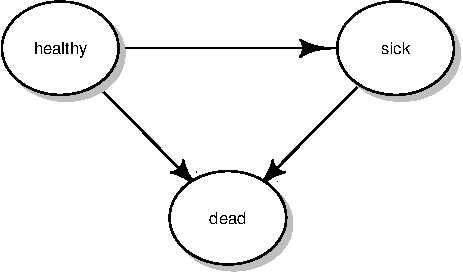
\includegraphics{VOI_toy_files/figure-latex/unnamed-chunk-4-1.pdf}

\hypertarget{incremental-nmb-inmb}{%
\section{04 Incremental NMB (INMB)}\label{incremental-nmb-inmb}}

\begin{Shaded}
\begin{Highlighting}[]
\CommentTok{# Calculate INMB of B vs A}
\CommentTok{# Only B vs A but we could have plotted all combinations}
\NormalTok{inmb <-}\StringTok{ }\KeywordTok{data.frame}\NormalTok{(}\DataTypeTok{Simulation =} \DecValTok{1}\OperatorTok{:}\NormalTok{n_sim,}
                   \StringTok{`}\DataTypeTok{Strategy B vs Strategy A}\StringTok{`}\NormalTok{ =}\StringTok{ }\NormalTok{nmb}\OperatorTok{$}\StringTok{`}\DataTypeTok{Strategy B}\StringTok{`} \OperatorTok{-}\StringTok{ }\NormalTok{nmb}\OperatorTok{$}\StringTok{`}\DataTypeTok{Strategy A}\StringTok{`}\NormalTok{) }

\CommentTok{## Format data frame suitably for plotting}
\NormalTok{inmb_gg <-}\StringTok{ }\KeywordTok{melt}\NormalTok{(inmb, }\DataTypeTok{id.vars =} \StringTok{"Simulation"}\NormalTok{, }
                \DataTypeTok{variable.name =} \StringTok{"Comparison"}\NormalTok{, }
                \DataTypeTok{value.name =} \StringTok{"INMB"}\NormalTok{)}
\NormalTok{txtsize <-}\StringTok{ }\DecValTok{16}

\CommentTok{## Plot INMB}
\KeywordTok{ggplot}\NormalTok{(inmb_gg, }\KeywordTok{aes}\NormalTok{(}\DataTypeTok{x =}\NormalTok{ INMB}\OperatorTok{/}\DecValTok{1000}\NormalTok{)) }\OperatorTok{+}
\StringTok{  }\KeywordTok{geom_histogram}\NormalTok{(}\KeywordTok{aes}\NormalTok{(}\DataTypeTok{y =}\NormalTok{..density..), }\DataTypeTok{col =} \StringTok{"black"}\NormalTok{, }\DataTypeTok{fill =} \StringTok{"gray"}\NormalTok{) }\OperatorTok{+}
\StringTok{  }\KeywordTok{geom_density}\NormalTok{(}\DataTypeTok{color =} \StringTok{"red"}\NormalTok{) }\OperatorTok{+}
\StringTok{  }\KeywordTok{geom_vline}\NormalTok{(}\DataTypeTok{xintercept =} \DecValTok{0}\NormalTok{, }\DataTypeTok{col =} \DecValTok{4}\NormalTok{, }\DataTypeTok{size =} \FloatTok{1.5}\NormalTok{, }\DataTypeTok{linetype =} \StringTok{"dashed"}\NormalTok{) }\OperatorTok{+}
\StringTok{  }\KeywordTok{facet_wrap}\NormalTok{(}\OperatorTok{~}\StringTok{ }\NormalTok{Comparison, }\DataTypeTok{scales =} \StringTok{"free_y"}\NormalTok{) }\OperatorTok{+}
\StringTok{  }\KeywordTok{xlab}\NormalTok{(}\StringTok{"Incremental Net Monetary Benefit (INMB) in thousand $"}\NormalTok{) }\OperatorTok{+}
\StringTok{  }\KeywordTok{scale_x_continuous}\NormalTok{(}\DataTypeTok{breaks =} \KeywordTok{number_ticks}\NormalTok{(}\DecValTok{5}\NormalTok{), }\DataTypeTok{limits =} \KeywordTok{c}\NormalTok{(}\OperatorTok{-}\DecValTok{100}\NormalTok{, }\DecValTok{100}\NormalTok{)) }\OperatorTok{+}\StringTok{ }
\StringTok{  }\KeywordTok{scale_y_continuous}\NormalTok{(}\DataTypeTok{breaks =} \KeywordTok{number_ticks}\NormalTok{(}\DecValTok{5}\NormalTok{)) }\OperatorTok{+}\StringTok{ }
\StringTok{  }\KeywordTok{theme_bw}\NormalTok{(}\DataTypeTok{base_size =} \DecValTok{14}\NormalTok{)}
\end{Highlighting}
\end{Shaded}

\begin{verbatim}
## `stat_bin()` using `bins = 30`. Pick better value with `binwidth`.
\end{verbatim}

\begin{verbatim}
## Warning: Removed 3 rows containing non-finite values (stat_bin).
\end{verbatim}

\begin{verbatim}
## Warning: Removed 3 rows containing non-finite values (stat_density).
\end{verbatim}

\begin{verbatim}
## Warning: Removed 1 rows containing missing values (geom_bar).
\end{verbatim}

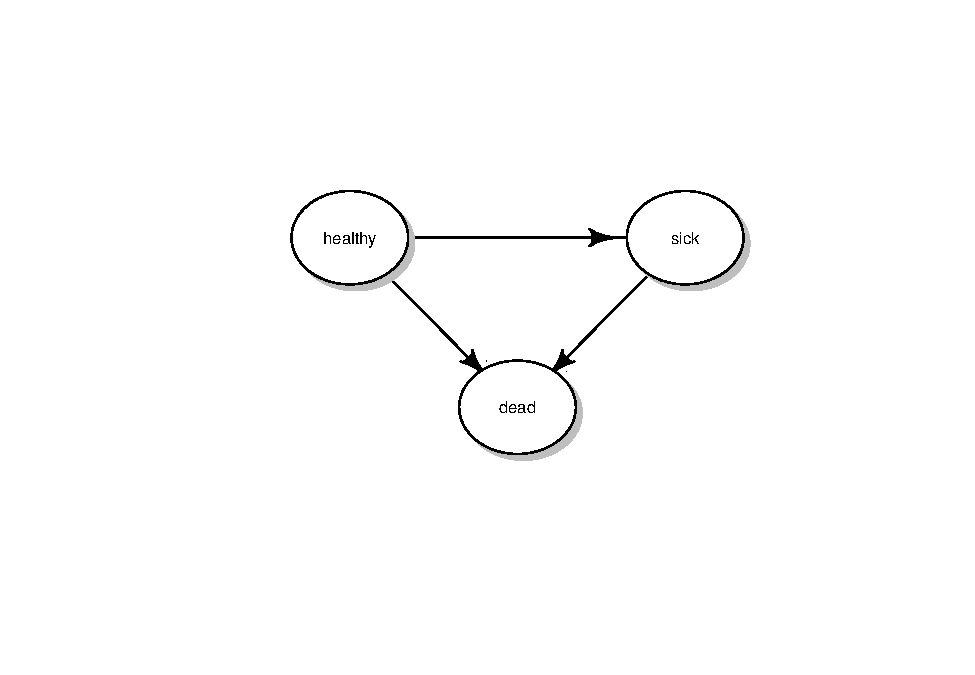
\includegraphics{VOI_toy_files/figure-latex/unnamed-chunk-5-1.pdf}

\hypertarget{loss-matrix}{%
\section{05 Loss Matrix}\label{loss-matrix}}

\begin{Shaded}
\begin{Highlighting}[]
\CommentTok{# Find optimal strategy (d*) based on the highest expected NMB}
\NormalTok{d_star <-}\StringTok{ }\KeywordTok{which.max}\NormalTok{(}\KeywordTok{colMeans}\NormalTok{(nmb))}
\NormalTok{d_star}
\end{Highlighting}
\end{Shaded}

\begin{verbatim}
## Strategy B 
##          2
\end{verbatim}

\begin{Shaded}
\begin{Highlighting}[]
\CommentTok{# Compute Loss matrix iterating over all strategies}
\CommentTok{# Initialize loss matrix of dimension: number of simulation by number of strategies}
\NormalTok{loss <-}\StringTok{ }\KeywordTok{matrix}\NormalTok{(}\DecValTok{0}\NormalTok{, n_sim, n_strategies)}
\ControlFlowTok{for}\NormalTok{ (d }\ControlFlowTok{in} \DecValTok{1}\OperatorTok{:}\NormalTok{n_strategies)\{ }\CommentTok{# d <- 1}
\NormalTok{  loss[, d] <-}\StringTok{ }\NormalTok{nmb[, d] }\OperatorTok{-}\StringTok{ }\NormalTok{nmb[, d_star]}
\NormalTok{\}}
\KeywordTok{head}\NormalTok{(loss)}
\end{Highlighting}
\end{Shaded}

\begin{verbatim}
##            [,1] [,2]        [,3]
## [1,]  -3727.713    0   -953.4139
## [2,]  -1608.355    0    276.6166
## [3,]  21574.683    0  -3345.1873
## [4,]  32212.210    0   2337.8737
## [5,]  17864.411    0   8466.6869
## [6,] -25717.410    0 -21012.2516
\end{verbatim}

\begin{Shaded}
\begin{Highlighting}[]
\CommentTok{# Or without iterating (much faster!)}
\NormalTok{loss <-}\StringTok{ }\KeywordTok{as.matrix}\NormalTok{(nmb }\OperatorTok{-}\StringTok{ }\NormalTok{nmb[, d_star])}
\KeywordTok{head}\NormalTok{(loss)}
\end{Highlighting}
\end{Shaded}

\begin{verbatim}
##      Strategy A Strategy B  Strategy C
## [1,]  -3727.713          0   -953.4139
## [2,]  -1608.355          0    276.6166
## [3,]  21574.683          0  -3345.1873
## [4,]  32212.210          0   2337.8737
## [5,]  17864.411          0   8466.6869
## [6,] -25717.410          0 -21012.2516
\end{verbatim}

\hypertarget{evpi}{%
\section{06 EVPI}\label{evpi}}

\begin{Shaded}
\begin{Highlighting}[]
\CommentTok{# Find maximum loss overall strategies at each state of the world }
\CommentTok{# (i.e., PSA sample)}
\NormalTok{max_loss_i <-}\StringTok{ }\KeywordTok{rowMaxs}\NormalTok{(loss)  }\CommentTok{# Only the positive values are a loss. Negative values show we selected the best strategy}
\KeywordTok{head}\NormalTok{(max_loss_i)}
\end{Highlighting}
\end{Shaded}

\begin{verbatim}
## [1]     0.0000   276.6166 21574.6828 32212.2103 17864.4110     0.0000
\end{verbatim}

\begin{Shaded}
\begin{Highlighting}[]
\CommentTok{## Average expected loss across all states of the world}
\CommentTok{## Expected loss = expected value of perfect information}
\NormalTok{evpi <-}\StringTok{ }\KeywordTok{mean}\NormalTok{(max_loss_i)}
\NormalTok{evpi}
\end{Highlighting}
\end{Shaded}

\begin{verbatim}
## [1] 5479.777
\end{verbatim}

\hypertarget{evppi}{%
\section{07 EVPPI}\label{evppi}}

\begin{Shaded}
\begin{Highlighting}[]
\NormalTok{names_params <-}\StringTok{ }\KeywordTok{c}\NormalTok{(}\StringTok{"Mean No. Visits (A)"}\NormalTok{, }
                   \StringTok{"Mean No. Visits (B)"}\NormalTok{,}
                   \StringTok{"Prob. Failing (A)"}\NormalTok{, }
                   \StringTok{"Prob. Failing (B)"}\NormalTok{)}
\CommentTok{# Matrix with parameters}
\NormalTok{x <-}\StringTok{ }\NormalTok{toy[, }\DecValTok{1}\OperatorTok{:}\DecValTok{4}\NormalTok{]}
\KeywordTok{colnames}\NormalTok{(x) <-}\StringTok{ }\NormalTok{names_params}
\KeywordTok{head}\NormalTok{(x)}
\end{Highlighting}
\end{Shaded}

\begin{verbatim}
##   Mean No. Visits (A) Mean No. Visits (B) Prob. Failing (A) Prob. Failing (B)
## 1           0.8878316            1.573204        0.22631182         0.4162887
## 2           1.1634753            2.131494        0.12227660         0.2878778
## 3           0.6734097            1.692781        0.05871254         0.3331618
## 4           0.6550782            2.066741        0.04683573         0.3558635
## 5           0.8545875            2.570651        0.09996313         0.3562357
## 6           0.5778263            1.329487        0.38803878         0.1979069
\end{verbatim}

\begin{Shaded}
\begin{Highlighting}[]
\CommentTok{# Number and names of parameters}
\NormalTok{n_params <-}\StringTok{ }\KeywordTok{ncol}\NormalTok{(x)}
\NormalTok{n_params}
\end{Highlighting}
\end{Shaded}

\begin{verbatim}
## [1] 4
\end{verbatim}

\begin{Shaded}
\begin{Highlighting}[]
\CommentTok{# Histogram of parameters}
\CommentTok{# Format data suitably for plotting}
\NormalTok{params <-}\StringTok{ }\KeywordTok{melt}\NormalTok{(x, }\DataTypeTok{variable.name =} \StringTok{"Parameter"}\NormalTok{)}
\end{Highlighting}
\end{Shaded}

\begin{verbatim}
## No id variables; using all as measure variables
\end{verbatim}

\begin{Shaded}
\begin{Highlighting}[]
\KeywordTok{head}\NormalTok{(params)}
\end{Highlighting}
\end{Shaded}

\begin{verbatim}
##             Parameter     value
## 1 Mean No. Visits (A) 0.8878316
## 2 Mean No. Visits (A) 1.1634753
## 3 Mean No. Visits (A) 0.6734097
## 4 Mean No. Visits (A) 0.6550782
## 5 Mean No. Visits (A) 0.8545875
## 6 Mean No. Visits (A) 0.5778263
\end{verbatim}

\begin{Shaded}
\begin{Highlighting}[]
\CommentTok{# Make parameter names as factors (helps with plotting formatting)}
\NormalTok{params}\OperatorTok{$}\NormalTok{Parameter <-}\StringTok{ }\KeywordTok{factor}\NormalTok{(params}\OperatorTok{$}\NormalTok{Parameter, }
                           \DataTypeTok{levels =}\NormalTok{ names_params, }
                           \DataTypeTok{labels =}\NormalTok{ names_params)}
\CommentTok{# Facet plot of parameter distributions}
\KeywordTok{ggplot}\NormalTok{(params, }\KeywordTok{aes}\NormalTok{(}\DataTypeTok{x =}\NormalTok{ value)) }\OperatorTok{+}\StringTok{ }
\StringTok{  }\KeywordTok{geom_histogram}\NormalTok{(}\KeywordTok{aes}\NormalTok{(}\DataTypeTok{y =}\NormalTok{..density..), }\DataTypeTok{col=}\StringTok{"black"}\NormalTok{, }\DataTypeTok{fill =} \StringTok{"gray"}\NormalTok{) }\OperatorTok{+}
\StringTok{  }\KeywordTok{geom_density}\NormalTok{(}\DataTypeTok{color =} \StringTok{"red"}\NormalTok{) }\OperatorTok{+}
\StringTok{  }\KeywordTok{facet_wrap}\NormalTok{(}\OperatorTok{~}\StringTok{ }\NormalTok{Parameter, }\DataTypeTok{scales =} \StringTok{"free"}\NormalTok{) }\OperatorTok{+}
\StringTok{  }\KeywordTok{scale_x_continuous}\NormalTok{(}\DataTypeTok{breaks =} \KeywordTok{number_ticks}\NormalTok{(}\DecValTok{5}\NormalTok{)) }\OperatorTok{+}\StringTok{ }
\StringTok{  }\KeywordTok{scale_y_continuous}\NormalTok{(}\DataTypeTok{breaks =} \KeywordTok{number_ticks}\NormalTok{(}\DecValTok{5}\NormalTok{)) }\OperatorTok{+}\StringTok{ }
\StringTok{  }\KeywordTok{theme_bw}\NormalTok{(}\DataTypeTok{base_size =} \DecValTok{14}\NormalTok{)}
\end{Highlighting}
\end{Shaded}

\begin{verbatim}
## `stat_bin()` using `bins = 30`. Pick better value with `binwidth`.
\end{verbatim}

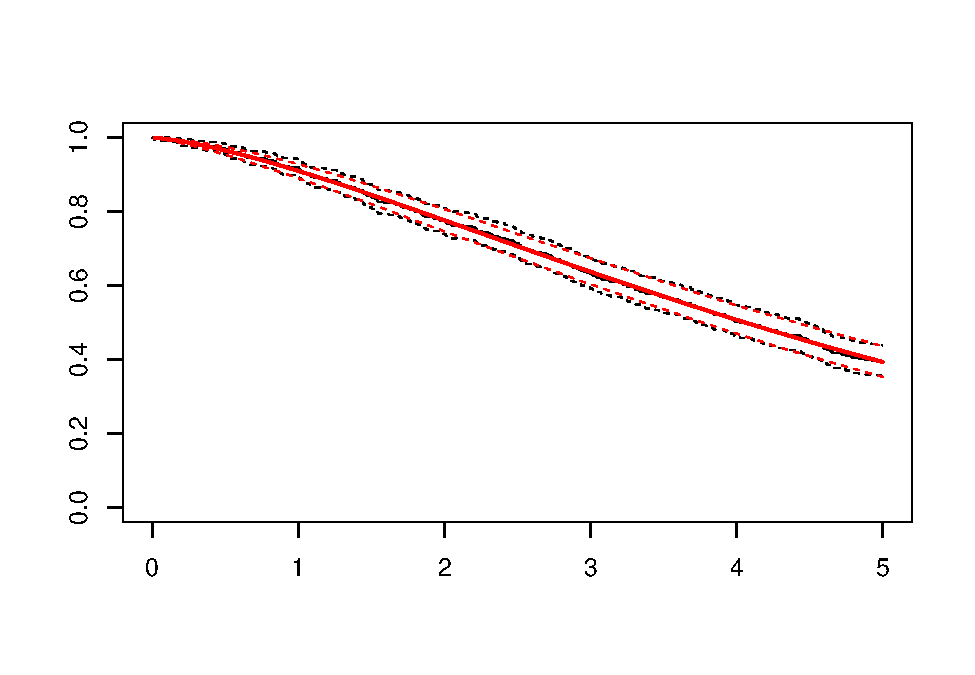
\includegraphics{VOI_toy_files/figure-latex/unnamed-chunk-8-1.pdf}

\hypertarget{construct-spline-metamodel}{%
\subsubsection{Construct Spline
metamodel}\label{construct-spline-metamodel}}

\begin{Shaded}
\begin{Highlighting}[]
\CommentTok{# Splines}
\CommentTok{# Initialize EVPPI vector }
\NormalTok{evppi_splines <-}\StringTok{ }\KeywordTok{matrix}\NormalTok{(}\DecValTok{0}\NormalTok{, n_params)}
\NormalTok{lmm1 <-}\StringTok{ }\KeywordTok{vector}\NormalTok{(}\StringTok{"list"}\NormalTok{, n_params)}
\NormalTok{lmm2 <-}\StringTok{ }\KeywordTok{vector}\NormalTok{(}\StringTok{"list"}\NormalTok{, n_params)}
\NormalTok{lmm3 <-}\StringTok{ }\KeywordTok{vector}\NormalTok{(}\StringTok{"list"}\NormalTok{, n_params)}
\ControlFlowTok{for}\NormalTok{ (p }\ControlFlowTok{in} \DecValTok{1}\OperatorTok{:}\NormalTok{n_params)\{ }\CommentTok{# p <- 1}
  \KeywordTok{print}\NormalTok{(}\KeywordTok{paste}\NormalTok{(}\StringTok{"Computing EVPPI of parameter"}\NormalTok{, names_params[p]))}
  \CommentTok{# Estimate Splines}
\NormalTok{  lmm1[[p]] <-}\StringTok{ }\KeywordTok{gam}\NormalTok{(loss[, }\DecValTok{1}\NormalTok{] }\OperatorTok{~}\StringTok{ }\KeywordTok{s}\NormalTok{(x[, p]))}
\NormalTok{  lmm2[[p]] <-}\StringTok{ }\KeywordTok{gam}\NormalTok{(loss[, }\DecValTok{2}\NormalTok{] }\OperatorTok{~}\StringTok{ }\KeywordTok{s}\NormalTok{(x[, p]))}
\NormalTok{  lmm3[[p]] <-}\StringTok{ }\KeywordTok{gam}\NormalTok{(loss[, }\DecValTok{2}\NormalTok{] }\OperatorTok{~}\StringTok{ }\KeywordTok{s}\NormalTok{(x[, p]))}
  
  \CommentTok{# Predict Loss using Splines}
\NormalTok{  Lhat_splines <-}\StringTok{ }\KeywordTok{cbind}\NormalTok{(lmm1[[p]]}\OperatorTok{$}\NormalTok{fitted, lmm2[[p]]}\OperatorTok{$}\NormalTok{fitted, lmm3[[p]]}\OperatorTok{$}\NormalTok{fitted)}
  
  \CommentTok{# Compute EVPPI}
\NormalTok{  evppi_splines[p] <-}\StringTok{ }\KeywordTok{mean}\NormalTok{(}\KeywordTok{rowMaxs}\NormalTok{(Lhat_splines))}
\NormalTok{\}}
\end{Highlighting}
\end{Shaded}

\begin{verbatim}
## [1] "Computing EVPPI of parameter Mean No. Visits (A)"
## [1] "Computing EVPPI of parameter Mean No. Visits (B)"
## [1] "Computing EVPPI of parameter Prob. Failing (A)"
## [1] "Computing EVPPI of parameter Prob. Failing (B)"
\end{verbatim}

\begin{Shaded}
\begin{Highlighting}[]
\CommentTok{# Ploting EVPPI using of order polynomial}
\NormalTok{evppi_splines_gg <-}\StringTok{ }\KeywordTok{data.frame}\NormalTok{(}\DataTypeTok{Parameter =}\NormalTok{ names_params, }\DataTypeTok{EVPPI =}\NormalTok{ evppi_splines)}
\NormalTok{evppi_splines_gg}\OperatorTok{$}\NormalTok{Parameter <-}\StringTok{ }\KeywordTok{factor}\NormalTok{((evppi_splines_gg}\OperatorTok{$}\NormalTok{Parameter), }
                              \DataTypeTok{levels =}\NormalTok{ names_params[}\KeywordTok{order}\NormalTok{(evppi_splines_gg}\OperatorTok{$}\NormalTok{EVPPI, }\DataTypeTok{decreasing =} \OtherTok{TRUE}\NormalTok{)])}

\CommentTok{# Plot EVPPI using ggplot2 package}
\KeywordTok{ggplot}\NormalTok{(}\DataTypeTok{data =}\NormalTok{ evppi_splines_gg, }\KeywordTok{aes}\NormalTok{(}\DataTypeTok{x =}\NormalTok{ Parameter, }\DataTypeTok{y =}\NormalTok{ EVPPI)) }\OperatorTok{+}
\StringTok{  }\KeywordTok{geom_bar}\NormalTok{(}\DataTypeTok{stat =} \StringTok{"identity"}\NormalTok{) }\OperatorTok{+}
\StringTok{  }\KeywordTok{ylab}\NormalTok{(}\StringTok{"EVPPI ($)"}\NormalTok{) }\OperatorTok{+}
\StringTok{  }\KeywordTok{scale_y_continuous}\NormalTok{(}\DataTypeTok{breaks =} \KeywordTok{number_ticks}\NormalTok{(}\DecValTok{6}\NormalTok{), }\DataTypeTok{labels =}\NormalTok{ comma) }\OperatorTok{+}
\StringTok{  }\KeywordTok{theme_bw}\NormalTok{(}\DataTypeTok{base_size =} \DecValTok{14}\NormalTok{)}
\end{Highlighting}
\end{Shaded}

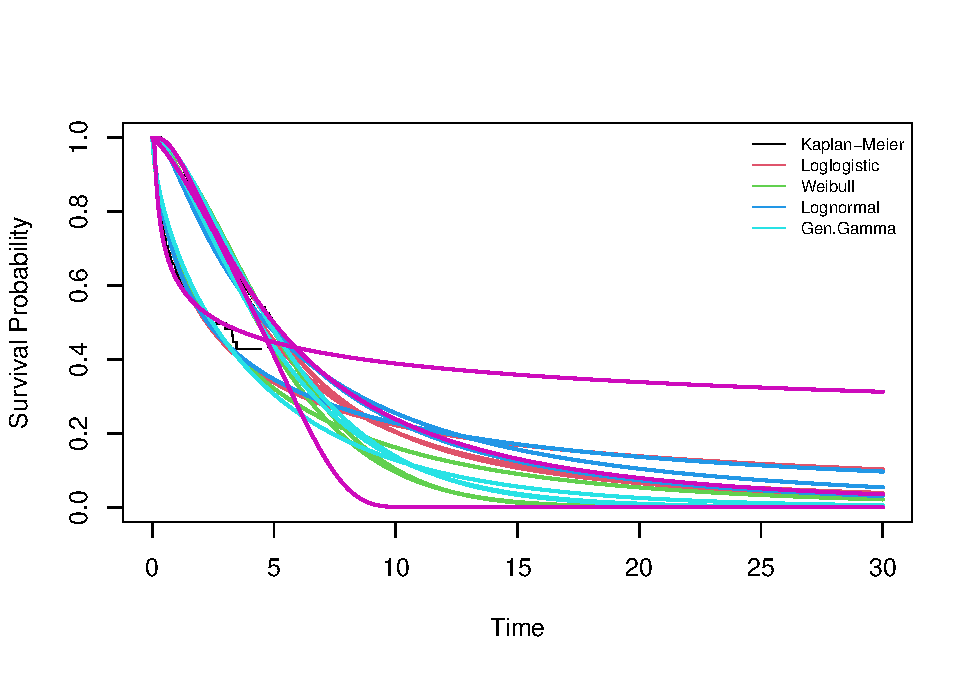
\includegraphics{VOI_toy_files/figure-latex/unnamed-chunk-9-1.pdf}

\hypertarget{expected-value-of-sample-information-evsi}{%
\section{08 Expected value of sample information
(EVSI)}\label{expected-value-of-sample-information-evsi}}

\begin{Shaded}
\begin{Highlighting}[]
\CommentTok{# Effective (prior) Sample size}
\NormalTok{n0 <-}\StringTok{ }\KeywordTok{c}\NormalTok{(}\DecValTok{10}\NormalTok{, }\CommentTok{# MeanNumVisitsA}
        \DecValTok{10}\NormalTok{, }\CommentTok{# MeanNumVisitsB}
        \DecValTok{10}\NormalTok{, }\CommentTok{# ProbFailA}
        \DecValTok{10}\NormalTok{) }\CommentTok{# ProbFailB}
\NormalTok{n <-}\StringTok{ }\KeywordTok{c}\NormalTok{(}\DecValTok{0}\NormalTok{, }\DecValTok{1}\NormalTok{, }\DecValTok{5}\NormalTok{, }\DecValTok{10}\NormalTok{, }\KeywordTok{seq}\NormalTok{(}\DecValTok{20}\NormalTok{, }\DecValTok{200}\NormalTok{, }\DataTypeTok{by =} \DecValTok{20}\NormalTok{))}
\NormalTok{n_samples <-}\StringTok{ }\KeywordTok{length}\NormalTok{(n)}

\CommentTok{# Each parameter individually (only assuming linear relationship)}
\CommentTok{# Initialize EVSI matrix for each parameters}
\NormalTok{evsi <-}\StringTok{ }\KeywordTok{data.frame}\NormalTok{(}\DataTypeTok{N =}\NormalTok{ n, }\KeywordTok{matrix}\NormalTok{(}\DecValTok{0}\NormalTok{, }\DataTypeTok{nrow =}\NormalTok{ n_samples, }\DataTypeTok{ncol =}\NormalTok{ n_params))}

\CommentTok{# Name columns of EVPSI matrix with parameter names}
\KeywordTok{colnames}\NormalTok{(evsi)[}\OperatorTok{-}\DecValTok{1}\NormalTok{] <-}\StringTok{ }\NormalTok{names_params}

\CommentTok{# Compute EVSI for all parameters separately}
\ControlFlowTok{for}\NormalTok{ (p }\ControlFlowTok{in} \DecValTok{1}\OperatorTok{:}\NormalTok{n_params)\{ }\CommentTok{# p <- 1}
  \KeywordTok{print}\NormalTok{(}\KeywordTok{paste}\NormalTok{(}\StringTok{"Computing EVSI of parameter"}\NormalTok{, names_params[p]))}
    \CommentTok{# Update loss based on gaussian approximation for each sample of interest}
    \ControlFlowTok{for}\NormalTok{ (nSamp }\ControlFlowTok{in} \DecValTok{1}\OperatorTok{:}\NormalTok{n_samples)\{ }\CommentTok{# nSamp <- 10}
\NormalTok{      Ltilde1 <-}\StringTok{ }\KeywordTok{predict.ga}\NormalTok{(lmm1[[p]], }\DataTypeTok{n =}\NormalTok{ n[nSamp], }\DataTypeTok{n0 =}\NormalTok{ n0[p])}
\NormalTok{      Ltilde2 <-}\StringTok{ }\KeywordTok{predict.ga}\NormalTok{(lmm2[[p]], }\DataTypeTok{n =}\NormalTok{ n[nSamp], }\DataTypeTok{n0 =}\NormalTok{ n0[p])}
\NormalTok{      Ltilde3 <-}\StringTok{ }\KeywordTok{predict.ga}\NormalTok{(lmm3[[p]], }\DataTypeTok{n =}\NormalTok{ n[nSamp], }\DataTypeTok{n0 =}\NormalTok{ n0[p])}
      \CommentTok{## Combine losses into one matrix}
\NormalTok{      Ltilde <-}\StringTok{ }\KeywordTok{cbind}\NormalTok{(Ltilde1, Ltilde2, Ltilde3)}
      \CommentTok{### Apply EVSI equation}
\NormalTok{      evsi[nSamp, p}\OperatorTok{+}\DecValTok{1}\NormalTok{] <-}\StringTok{ }\KeywordTok{mean}\NormalTok{(}\KeywordTok{rowMaxs}\NormalTok{(Ltilde))}
\NormalTok{    \}}
\NormalTok{\}}
\end{Highlighting}
\end{Shaded}

\begin{verbatim}
## [1] "Computing EVSI of parameter Mean No. Visits (A)"
## [1] "Variance reduction factor = 0"
## [1] "Variance reduction factor = 0"
## [1] "Variance reduction factor = 0"
## [1] "Variance reduction factor = 0.302"
## [1] "Variance reduction factor = 0.302"
## [1] "Variance reduction factor = 0.302"
## [1] "Variance reduction factor = 0.577"
## [1] "Variance reduction factor = 0.577"
## [1] "Variance reduction factor = 0.577"
## [1] "Variance reduction factor = 0.707"
## [1] "Variance reduction factor = 0.707"
## [1] "Variance reduction factor = 0.707"
## [1] "Variance reduction factor = 0.816"
## [1] "Variance reduction factor = 0.816"
## [1] "Variance reduction factor = 0.816"
## [1] "Variance reduction factor = 0.894"
## [1] "Variance reduction factor = 0.894"
## [1] "Variance reduction factor = 0.894"
## [1] "Variance reduction factor = 0.926"
## [1] "Variance reduction factor = 0.926"
## [1] "Variance reduction factor = 0.926"
## [1] "Variance reduction factor = 0.943"
## [1] "Variance reduction factor = 0.943"
## [1] "Variance reduction factor = 0.943"
## [1] "Variance reduction factor = 0.953"
## [1] "Variance reduction factor = 0.953"
## [1] "Variance reduction factor = 0.953"
## [1] "Variance reduction factor = 0.961"
## [1] "Variance reduction factor = 0.961"
## [1] "Variance reduction factor = 0.961"
## [1] "Variance reduction factor = 0.966"
## [1] "Variance reduction factor = 0.966"
## [1] "Variance reduction factor = 0.966"
## [1] "Variance reduction factor = 0.97"
## [1] "Variance reduction factor = 0.97"
## [1] "Variance reduction factor = 0.97"
## [1] "Variance reduction factor = 0.973"
## [1] "Variance reduction factor = 0.973"
## [1] "Variance reduction factor = 0.973"
## [1] "Variance reduction factor = 0.976"
## [1] "Variance reduction factor = 0.976"
## [1] "Variance reduction factor = 0.976"
## [1] "Computing EVSI of parameter Mean No. Visits (B)"
## [1] "Variance reduction factor = 0"
## [1] "Variance reduction factor = 0"
## [1] "Variance reduction factor = 0"
## [1] "Variance reduction factor = 0.302"
## [1] "Variance reduction factor = 0.302"
## [1] "Variance reduction factor = 0.302"
## [1] "Variance reduction factor = 0.577"
## [1] "Variance reduction factor = 0.577"
## [1] "Variance reduction factor = 0.577"
## [1] "Variance reduction factor = 0.707"
## [1] "Variance reduction factor = 0.707"
## [1] "Variance reduction factor = 0.707"
## [1] "Variance reduction factor = 0.816"
## [1] "Variance reduction factor = 0.816"
## [1] "Variance reduction factor = 0.816"
## [1] "Variance reduction factor = 0.894"
## [1] "Variance reduction factor = 0.894"
## [1] "Variance reduction factor = 0.894"
## [1] "Variance reduction factor = 0.926"
## [1] "Variance reduction factor = 0.926"
## [1] "Variance reduction factor = 0.926"
## [1] "Variance reduction factor = 0.943"
## [1] "Variance reduction factor = 0.943"
## [1] "Variance reduction factor = 0.943"
## [1] "Variance reduction factor = 0.953"
## [1] "Variance reduction factor = 0.953"
## [1] "Variance reduction factor = 0.953"
## [1] "Variance reduction factor = 0.961"
## [1] "Variance reduction factor = 0.961"
## [1] "Variance reduction factor = 0.961"
## [1] "Variance reduction factor = 0.966"
## [1] "Variance reduction factor = 0.966"
## [1] "Variance reduction factor = 0.966"
## [1] "Variance reduction factor = 0.97"
## [1] "Variance reduction factor = 0.97"
## [1] "Variance reduction factor = 0.97"
## [1] "Variance reduction factor = 0.973"
## [1] "Variance reduction factor = 0.973"
## [1] "Variance reduction factor = 0.973"
## [1] "Variance reduction factor = 0.976"
## [1] "Variance reduction factor = 0.976"
## [1] "Variance reduction factor = 0.976"
## [1] "Computing EVSI of parameter Prob. Failing (A)"
## [1] "Variance reduction factor = 0"
## [1] "Variance reduction factor = 0"
## [1] "Variance reduction factor = 0"
## [1] "Variance reduction factor = 0.302"
## [1] "Variance reduction factor = 0.302"
## [1] "Variance reduction factor = 0.302"
## [1] "Variance reduction factor = 0.577"
## [1] "Variance reduction factor = 0.577"
## [1] "Variance reduction factor = 0.577"
## [1] "Variance reduction factor = 0.707"
## [1] "Variance reduction factor = 0.707"
## [1] "Variance reduction factor = 0.707"
## [1] "Variance reduction factor = 0.816"
## [1] "Variance reduction factor = 0.816"
## [1] "Variance reduction factor = 0.816"
## [1] "Variance reduction factor = 0.894"
## [1] "Variance reduction factor = 0.894"
## [1] "Variance reduction factor = 0.894"
## [1] "Variance reduction factor = 0.926"
## [1] "Variance reduction factor = 0.926"
## [1] "Variance reduction factor = 0.926"
## [1] "Variance reduction factor = 0.943"
## [1] "Variance reduction factor = 0.943"
## [1] "Variance reduction factor = 0.943"
## [1] "Variance reduction factor = 0.953"
## [1] "Variance reduction factor = 0.953"
## [1] "Variance reduction factor = 0.953"
## [1] "Variance reduction factor = 0.961"
## [1] "Variance reduction factor = 0.961"
## [1] "Variance reduction factor = 0.961"
## [1] "Variance reduction factor = 0.966"
## [1] "Variance reduction factor = 0.966"
## [1] "Variance reduction factor = 0.966"
## [1] "Variance reduction factor = 0.97"
## [1] "Variance reduction factor = 0.97"
## [1] "Variance reduction factor = 0.97"
## [1] "Variance reduction factor = 0.973"
## [1] "Variance reduction factor = 0.973"
## [1] "Variance reduction factor = 0.973"
## [1] "Variance reduction factor = 0.976"
## [1] "Variance reduction factor = 0.976"
## [1] "Variance reduction factor = 0.976"
## [1] "Computing EVSI of parameter Prob. Failing (B)"
## [1] "Variance reduction factor = 0"
## [1] "Variance reduction factor = 0"
## [1] "Variance reduction factor = 0"
## [1] "Variance reduction factor = 0.302"
## [1] "Variance reduction factor = 0.302"
## [1] "Variance reduction factor = 0.302"
## [1] "Variance reduction factor = 0.577"
## [1] "Variance reduction factor = 0.577"
## [1] "Variance reduction factor = 0.577"
## [1] "Variance reduction factor = 0.707"
## [1] "Variance reduction factor = 0.707"
## [1] "Variance reduction factor = 0.707"
## [1] "Variance reduction factor = 0.816"
## [1] "Variance reduction factor = 0.816"
## [1] "Variance reduction factor = 0.816"
## [1] "Variance reduction factor = 0.894"
## [1] "Variance reduction factor = 0.894"
## [1] "Variance reduction factor = 0.894"
## [1] "Variance reduction factor = 0.926"
## [1] "Variance reduction factor = 0.926"
## [1] "Variance reduction factor = 0.926"
## [1] "Variance reduction factor = 0.943"
## [1] "Variance reduction factor = 0.943"
## [1] "Variance reduction factor = 0.943"
## [1] "Variance reduction factor = 0.953"
## [1] "Variance reduction factor = 0.953"
## [1] "Variance reduction factor = 0.953"
## [1] "Variance reduction factor = 0.961"
## [1] "Variance reduction factor = 0.961"
## [1] "Variance reduction factor = 0.961"
## [1] "Variance reduction factor = 0.966"
## [1] "Variance reduction factor = 0.966"
## [1] "Variance reduction factor = 0.966"
## [1] "Variance reduction factor = 0.97"
## [1] "Variance reduction factor = 0.97"
## [1] "Variance reduction factor = 0.97"
## [1] "Variance reduction factor = 0.973"
## [1] "Variance reduction factor = 0.973"
## [1] "Variance reduction factor = 0.973"
## [1] "Variance reduction factor = 0.976"
## [1] "Variance reduction factor = 0.976"
## [1] "Variance reduction factor = 0.976"
\end{verbatim}

\begin{Shaded}
\begin{Highlighting}[]
\CommentTok{# Plotting EVSI}
\CommentTok{# Create EVSI data frame for plotting in decreasing order of EVPPI}
\NormalTok{evsi_gg <-}\StringTok{ }\KeywordTok{melt}\NormalTok{(evsi[}\DecValTok{1}\OperatorTok{:}\DecValTok{21}\NormalTok{,], }\DataTypeTok{id.vars =} \StringTok{"N"}\NormalTok{, }
                 \DataTypeTok{variable.name =} \StringTok{"Parameter"}\NormalTok{, }
                 \DataTypeTok{value.name =} \StringTok{"evsi"}\NormalTok{)}
\NormalTok{evsi_gg}\OperatorTok{$}\NormalTok{Parameter <-}\StringTok{ }\KeywordTok{factor}\NormalTok{((evsi_gg}\OperatorTok{$}\NormalTok{Parameter), }
                             \DataTypeTok{levels =}\NormalTok{ names_params[}\KeywordTok{order}\NormalTok{(evppi_splines_gg}\OperatorTok{$}\NormalTok{EVPPI, }\DataTypeTok{decreasing =} \OtherTok{TRUE}\NormalTok{)])}

\CommentTok{# Plot evsi using ggplot2 package}
\KeywordTok{ggplot}\NormalTok{(evsi_gg, }\KeywordTok{aes}\NormalTok{(}\DataTypeTok{x =}\NormalTok{ N, }\DataTypeTok{y =}\NormalTok{ evsi)) }\OperatorTok{+}\StringTok{  }\CommentTok{# colour = Parameter}
\StringTok{  }\KeywordTok{geom_line}\NormalTok{() }\OperatorTok{+}
\StringTok{  }\KeywordTok{geom_point}\NormalTok{() }\OperatorTok{+}
\StringTok{  }\KeywordTok{facet_wrap}\NormalTok{(}\OperatorTok{~}\StringTok{ }\NormalTok{Parameter) }\OperatorTok{+}\StringTok{  }\CommentTok{# scales = "free_y"}
\StringTok{  }\KeywordTok{ggtitle}\NormalTok{(}\StringTok{"Expected Value of Sample Information (EVSI)"}\NormalTok{) }\OperatorTok{+}
\StringTok{  }\KeywordTok{xlab}\NormalTok{(}\StringTok{"Sample size (n)"}\NormalTok{) }\OperatorTok{+}
\StringTok{  }\KeywordTok{ylab}\NormalTok{(}\StringTok{"$"}\NormalTok{) }\OperatorTok{+}
\StringTok{  }\KeywordTok{scale_x_continuous}\NormalTok{(}\DataTypeTok{breaks =} \KeywordTok{number_ticks}\NormalTok{(}\DecValTok{5}\NormalTok{)) }\OperatorTok{+}\StringTok{ }
\StringTok{  }\KeywordTok{scale_y_continuous}\NormalTok{(}\DataTypeTok{breaks =} \KeywordTok{number_ticks}\NormalTok{(}\DecValTok{6}\NormalTok{), }\DataTypeTok{labels =}\NormalTok{ dollar) }\OperatorTok{+}\StringTok{ }
\StringTok{  }\KeywordTok{theme_bw}\NormalTok{(}\DataTypeTok{base_size =} \DecValTok{14}\NormalTok{)}
\end{Highlighting}
\end{Shaded}

\begin{verbatim}
## Warning: Removed 7 row(s) containing missing values (geom_path).
\end{verbatim}

\begin{verbatim}
## Warning: Removed 28 rows containing missing values (geom_point).
\end{verbatim}

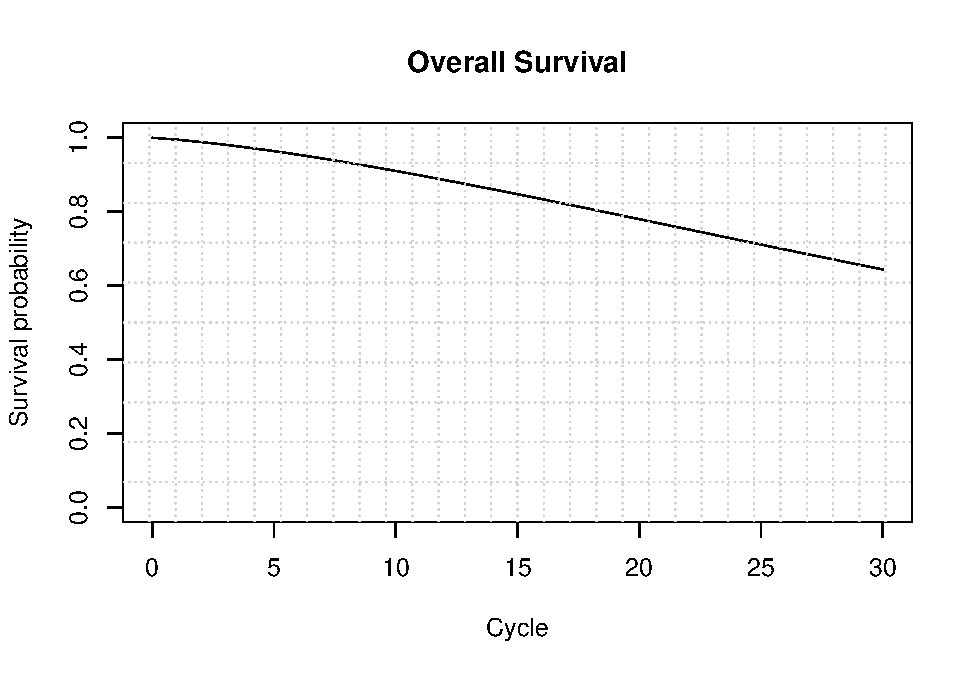
\includegraphics{VOI_toy_files/figure-latex/unnamed-chunk-10-1.pdf}

\begin{Shaded}
\begin{Highlighting}[]
\CommentTok{# Adding EVPPI }
\KeywordTok{ggplot}\NormalTok{(evsi_gg, }\KeywordTok{aes}\NormalTok{(}\DataTypeTok{x =}\NormalTok{ N, }\DataTypeTok{y =}\NormalTok{ evsi)) }\OperatorTok{+}\StringTok{  }\CommentTok{# colour = Parameter}
\StringTok{  }\KeywordTok{geom_line}\NormalTok{(}\KeywordTok{aes}\NormalTok{(}\DataTypeTok{linetype =} \StringTok{"EVSI"}\NormalTok{)) }\OperatorTok{+}
\StringTok{  }\KeywordTok{geom_point}\NormalTok{() }\OperatorTok{+}
\StringTok{  }\KeywordTok{facet_wrap}\NormalTok{(}\OperatorTok{~}\StringTok{ }\NormalTok{Parameter) }\OperatorTok{+}\StringTok{  }\CommentTok{# scales = "free_y"}
\StringTok{  }\KeywordTok{geom_hline}\NormalTok{(}\KeywordTok{aes}\NormalTok{(}\DataTypeTok{yintercept =}\NormalTok{ EVPPI, }\DataTypeTok{linetype =} \StringTok{"EVPPI"}\NormalTok{), }\DataTypeTok{data =}\NormalTok{ evppi_splines_gg) }\OperatorTok{+}
\StringTok{  }\KeywordTok{scale_linetype_manual}\NormalTok{(}\DataTypeTok{name=}\StringTok{""}\NormalTok{, }
                        \DataTypeTok{values =} \KeywordTok{c}\NormalTok{(}\StringTok{"EVSI"}\NormalTok{ =}\StringTok{ "solid"}\NormalTok{, }\StringTok{"EVPPI"}\NormalTok{ =}\StringTok{ "dashed"}\NormalTok{)) }\OperatorTok{+}
\StringTok{  }\KeywordTok{xlab}\NormalTok{(}\StringTok{"Sample size (n)"}\NormalTok{) }\OperatorTok{+}
\StringTok{  }\KeywordTok{ylab}\NormalTok{(}\StringTok{"$"}\NormalTok{) }\OperatorTok{+}
\StringTok{  }\CommentTok{#ggtitle("Expected Value of Sample Information (EVSI)") +}
\StringTok{  }\KeywordTok{scale_x_continuous}\NormalTok{(}\DataTypeTok{breaks =} \KeywordTok{number_ticks}\NormalTok{(}\DecValTok{5}\NormalTok{)) }\OperatorTok{+}\StringTok{ }
\StringTok{  }\KeywordTok{scale_y_continuous}\NormalTok{(}\DataTypeTok{breaks =} \KeywordTok{number_ticks}\NormalTok{(}\DecValTok{6}\NormalTok{), }\DataTypeTok{labels =}\NormalTok{ dollar) }\OperatorTok{+}\StringTok{ }
\StringTok{  }\KeywordTok{theme_bw}\NormalTok{(}\DataTypeTok{base_size =} \DecValTok{14}\NormalTok{)}
\end{Highlighting}
\end{Shaded}

\begin{verbatim}
## Warning: Removed 7 row(s) containing missing values (geom_path).

## Warning: Removed 28 rows containing missing values (geom_point).
\end{verbatim}

\includegraphics{VOI_toy_files/figure-latex/unnamed-chunk-10-2.pdf}

\hypertarget{combination-of-parameters}{%
\section{09 Combination of parameters}\label{combination-of-parameters}}

\hypertarget{assuming-an-observational-study}{%
\subsection{09.1 Assuming an observational
study}\label{assuming-an-observational-study}}

\begin{Shaded}
\begin{Highlighting}[]
\NormalTok{sel_params_obs <-}\StringTok{ }\KeywordTok{c}\NormalTok{(}\DecValTok{1}\NormalTok{, }\DecValTok{2}\NormalTok{)}
\CommentTok{# Vector with samples to evaluate EVPSI for an Observational design}
\NormalTok{n_obs <-}\StringTok{ }\KeywordTok{c}\NormalTok{(}\DecValTok{0}\NormalTok{, }\DecValTok{1}\NormalTok{, }\DecValTok{5}\NormalTok{, }\DecValTok{10}\NormalTok{, }\KeywordTok{seq}\NormalTok{(}\DecValTok{20}\NormalTok{, }\DecValTok{200}\NormalTok{, }\DataTypeTok{by =} \DecValTok{20}\NormalTok{), }\DecValTok{300}\NormalTok{, }\DecValTok{400}\NormalTok{, }\DecValTok{500}\NormalTok{, }\DecValTok{600}\NormalTok{, }\DecValTok{700}\NormalTok{, }\DecValTok{800}\NormalTok{) }\CommentTok{#seq(0, 1000, by = 20)}
\NormalTok{n_obs_samples <-}\StringTok{ }\KeywordTok{length}\NormalTok{(n_obs)}
\CommentTok{# Initailize EVPSI matrix for a combination of parameters}
\NormalTok{evsi_obs <-}\StringTok{ }\KeywordTok{data.frame}\NormalTok{(}\DataTypeTok{Study =} \StringTok{"Observational"}\NormalTok{, }
                        \DataTypeTok{N =}\NormalTok{ n_obs, }
                        \DataTypeTok{EVSI =} \KeywordTok{matrix}\NormalTok{(}\DecValTok{0}\NormalTok{, }\DataTypeTok{nrow =}\NormalTok{ n_obs_samples, }\DataTypeTok{ncol =} \DecValTok{1}\NormalTok{))}

\CommentTok{# Estimate linear metamodel of two parameters}
\NormalTok{lmm1_obs <-}\StringTok{ }\KeywordTok{gam}\NormalTok{(loss[, }\DecValTok{1}\NormalTok{] }\OperatorTok{~}\StringTok{ }\KeywordTok{s}\NormalTok{(x[, sel_params_obs[}\DecValTok{1}\NormalTok{]]) }\OperatorTok{+}\StringTok{ }
\StringTok{              }\KeywordTok{s}\NormalTok{(x[, sel_params_obs[}\DecValTok{2}\NormalTok{]]) }\OperatorTok{+}\StringTok{ }
\StringTok{              }\KeywordTok{ti}\NormalTok{(x[, sel_params_obs[}\DecValTok{1}\NormalTok{]], x[, sel_params_obs[}\DecValTok{2}\NormalTok{]]))}
\NormalTok{lmm2_obs <-}\StringTok{ }\KeywordTok{gam}\NormalTok{(loss[, }\DecValTok{2}\NormalTok{] }\OperatorTok{~}\StringTok{ }\KeywordTok{s}\NormalTok{(x[, sel_params_obs[}\DecValTok{1}\NormalTok{]]) }\OperatorTok{+}\StringTok{ }
\StringTok{                  }\KeywordTok{s}\NormalTok{(x[, sel_params_obs[}\DecValTok{2}\NormalTok{]]) }\OperatorTok{+}\StringTok{ }
\StringTok{                  }\KeywordTok{ti}\NormalTok{(x[, sel_params_obs[}\DecValTok{1}\NormalTok{]], x[, sel_params_obs[}\DecValTok{2}\NormalTok{]]))}
\NormalTok{lmm3_obs <-}\StringTok{ }\KeywordTok{gam}\NormalTok{(loss[, }\DecValTok{3}\NormalTok{] }\OperatorTok{~}\StringTok{ }\KeywordTok{s}\NormalTok{(x[, sel_params_obs[}\DecValTok{1}\NormalTok{]]) }\OperatorTok{+}\StringTok{ }
\StringTok{                  }\KeywordTok{s}\NormalTok{(x[, sel_params_obs[}\DecValTok{2}\NormalTok{]]) }\OperatorTok{+}\StringTok{ }
\StringTok{                  }\KeywordTok{ti}\NormalTok{(x[, sel_params_obs[}\DecValTok{1}\NormalTok{]], x[, sel_params_obs[}\DecValTok{2}\NormalTok{]]))}
\CommentTok{# Predict Loss using Splines}
\NormalTok{Lhat_obs_splines <-}\StringTok{ }\KeywordTok{cbind}\NormalTok{(lmm1_obs}\OperatorTok{$}\NormalTok{fitted, lmm2_obs}\OperatorTok{$}\NormalTok{fitted, lmm3_obs}\OperatorTok{$}\NormalTok{fitted)}

\CommentTok{# Compute EVPPI}
\NormalTok{evppi_obs <-}\StringTok{ }\KeywordTok{mean}\NormalTok{(}\KeywordTok{rowMaxs}\NormalTok{(Lhat_obs_splines))}
\NormalTok{evppi_obs          }
\end{Highlighting}
\end{Shaded}

\begin{verbatim}
## [1] 2621.822
\end{verbatim}

\begin{Shaded}
\begin{Highlighting}[]
\ControlFlowTok{for}\NormalTok{ (nSamp }\ControlFlowTok{in} \DecValTok{1}\OperatorTok{:}\NormalTok{n_obs_samples)\{}
\NormalTok{  Ltilde1_obs <-}\StringTok{ }\KeywordTok{predict.ga}\NormalTok{(lmm1_obs, }\DataTypeTok{n =}\NormalTok{ n_obs[nSamp], }\DataTypeTok{n0 =}\NormalTok{ n0[sel_params_obs])}
\NormalTok{  Ltilde2_obs <-}\StringTok{ }\KeywordTok{predict.ga}\NormalTok{(lmm2_obs, }\DataTypeTok{n =}\NormalTok{ n_obs[nSamp], }\DataTypeTok{n0 =}\NormalTok{ n0[sel_params_obs])}
\NormalTok{  Ltilde3_obs <-}\StringTok{ }\KeywordTok{predict.ga}\NormalTok{(lmm3_obs, }\DataTypeTok{n =}\NormalTok{ n_obs[nSamp], }\DataTypeTok{n0 =}\NormalTok{ n0[sel_params_obs])}
  \CommentTok{# Combine losses into one matrix}
\NormalTok{  Ltilde_obs <-}\StringTok{ }\KeywordTok{cbind}\NormalTok{(Ltilde1_obs, Ltilde2_obs, Ltilde3_obs)}
  \CommentTok{# Apply EVSI equation}
\NormalTok{  evsi_obs}\OperatorTok{$}\NormalTok{EVSI[nSamp] <-}\StringTok{ }\KeywordTok{mean}\NormalTok{(}\KeywordTok{rowMaxs}\NormalTok{(Ltilde_obs))}
\NormalTok{\}}
\end{Highlighting}
\end{Shaded}

\begin{verbatim}
## [1] "Variance reduction factor = 0" "Variance reduction factor = 0"
## [1] "Variance reduction factor = 0" "Variance reduction factor = 0"
## [1] "Variance reduction factor = 0" "Variance reduction factor = 0"
## [1] "Variance reduction factor = 0.302" "Variance reduction factor = 0.302"
## [1] "Variance reduction factor = 0.302" "Variance reduction factor = 0.302"
## [1] "Variance reduction factor = 0.302" "Variance reduction factor = 0.302"
## [1] "Variance reduction factor = 0.577" "Variance reduction factor = 0.577"
## [1] "Variance reduction factor = 0.577" "Variance reduction factor = 0.577"
## [1] "Variance reduction factor = 0.577" "Variance reduction factor = 0.577"
## [1] "Variance reduction factor = 0.707" "Variance reduction factor = 0.707"
## [1] "Variance reduction factor = 0.707" "Variance reduction factor = 0.707"
## [1] "Variance reduction factor = 0.707" "Variance reduction factor = 0.707"
## [1] "Variance reduction factor = 0.816" "Variance reduction factor = 0.816"
## [1] "Variance reduction factor = 0.816" "Variance reduction factor = 0.816"
## [1] "Variance reduction factor = 0.816" "Variance reduction factor = 0.816"
## [1] "Variance reduction factor = 0.894" "Variance reduction factor = 0.894"
## [1] "Variance reduction factor = 0.894" "Variance reduction factor = 0.894"
## [1] "Variance reduction factor = 0.894" "Variance reduction factor = 0.894"
## [1] "Variance reduction factor = 0.926" "Variance reduction factor = 0.926"
## [1] "Variance reduction factor = 0.926" "Variance reduction factor = 0.926"
## [1] "Variance reduction factor = 0.926" "Variance reduction factor = 0.926"
## [1] "Variance reduction factor = 0.943" "Variance reduction factor = 0.943"
## [1] "Variance reduction factor = 0.943" "Variance reduction factor = 0.943"
## [1] "Variance reduction factor = 0.943" "Variance reduction factor = 0.943"
## [1] "Variance reduction factor = 0.953" "Variance reduction factor = 0.953"
## [1] "Variance reduction factor = 0.953" "Variance reduction factor = 0.953"
## [1] "Variance reduction factor = 0.953" "Variance reduction factor = 0.953"
## [1] "Variance reduction factor = 0.961" "Variance reduction factor = 0.961"
## [1] "Variance reduction factor = 0.961" "Variance reduction factor = 0.961"
## [1] "Variance reduction factor = 0.961" "Variance reduction factor = 0.961"
## [1] "Variance reduction factor = 0.966" "Variance reduction factor = 0.966"
## [1] "Variance reduction factor = 0.966" "Variance reduction factor = 0.966"
## [1] "Variance reduction factor = 0.966" "Variance reduction factor = 0.966"
## [1] "Variance reduction factor = 0.97" "Variance reduction factor = 0.97"
## [1] "Variance reduction factor = 0.97" "Variance reduction factor = 0.97"
## [1] "Variance reduction factor = 0.97" "Variance reduction factor = 0.97"
## [1] "Variance reduction factor = 0.973" "Variance reduction factor = 0.973"
## [1] "Variance reduction factor = 0.973" "Variance reduction factor = 0.973"
## [1] "Variance reduction factor = 0.973" "Variance reduction factor = 0.973"
## [1] "Variance reduction factor = 0.976" "Variance reduction factor = 0.976"
## [1] "Variance reduction factor = 0.976" "Variance reduction factor = 0.976"
## [1] "Variance reduction factor = 0.976" "Variance reduction factor = 0.976"
## [1] "Variance reduction factor = 0.984" "Variance reduction factor = 0.984"
## [1] "Variance reduction factor = 0.984" "Variance reduction factor = 0.984"
## [1] "Variance reduction factor = 0.984" "Variance reduction factor = 0.984"
## [1] "Variance reduction factor = 0.988" "Variance reduction factor = 0.988"
## [1] "Variance reduction factor = 0.988" "Variance reduction factor = 0.988"
## [1] "Variance reduction factor = 0.988" "Variance reduction factor = 0.988"
## [1] "Variance reduction factor = 0.99" "Variance reduction factor = 0.99"
## [1] "Variance reduction factor = 0.99" "Variance reduction factor = 0.99"
## [1] "Variance reduction factor = 0.99" "Variance reduction factor = 0.99"
## [1] "Variance reduction factor = 0.992" "Variance reduction factor = 0.992"
## [1] "Variance reduction factor = 0.992" "Variance reduction factor = 0.992"
## [1] "Variance reduction factor = 0.992" "Variance reduction factor = 0.992"
## [1] "Variance reduction factor = 0.993" "Variance reduction factor = 0.993"
## [1] "Variance reduction factor = 0.993" "Variance reduction factor = 0.993"
## [1] "Variance reduction factor = 0.993" "Variance reduction factor = 0.993"
## [1] "Variance reduction factor = 0.994" "Variance reduction factor = 0.994"
## [1] "Variance reduction factor = 0.994" "Variance reduction factor = 0.994"
## [1] "Variance reduction factor = 0.994" "Variance reduction factor = 0.994"
\end{verbatim}

\hypertarget{assuming-an-rct}{%
\subsection{09.2 Assuming an RCT}\label{assuming-an-rct}}

\begin{Shaded}
\begin{Highlighting}[]
\NormalTok{sel_params_rct <-}\StringTok{ }\KeywordTok{c}\NormalTok{(}\DecValTok{3}\NormalTok{, }\DecValTok{4}\NormalTok{)}
\CommentTok{# Vector with samples to evaluate EVPSI for a RCT}
\NormalTok{n_rct <-}\StringTok{ }\KeywordTok{c}\NormalTok{(}\DecValTok{0}\NormalTok{, }\DecValTok{1}\NormalTok{, }\DecValTok{5}\NormalTok{, }\DecValTok{10}\NormalTok{, }\KeywordTok{seq}\NormalTok{(}\DecValTok{20}\NormalTok{, }\DecValTok{200}\NormalTok{, }\DataTypeTok{by =} \DecValTok{20}\NormalTok{))}
\NormalTok{n_rct_samples <-}\StringTok{ }\KeywordTok{length}\NormalTok{(n_rct)}
\CommentTok{# Initailize EVPSI matrix for a combination of parameters}
\NormalTok{evsi_rct <-}\StringTok{ }\KeywordTok{data.frame}\NormalTok{(}\DataTypeTok{Study =} \StringTok{"RCT"}\NormalTok{,}
                        \DataTypeTok{N =}\NormalTok{ n_rct, }
                        \DataTypeTok{EVSI =} \KeywordTok{matrix}\NormalTok{(}\DecValTok{0}\NormalTok{, }\DataTypeTok{nrow =}\NormalTok{ n_rct_samples, }\DataTypeTok{ncol =} \DecValTok{1}\NormalTok{))}

\CommentTok{# Estimate linear metamodel of two parameters}
\NormalTok{lmm1_rct <-}\StringTok{ }\KeywordTok{gam}\NormalTok{(loss[, }\DecValTok{1}\NormalTok{] }\OperatorTok{~}\StringTok{ }\KeywordTok{s}\NormalTok{(x[, sel_params_rct[}\DecValTok{1}\NormalTok{]]) }\OperatorTok{+}\StringTok{ }
\StringTok{                  }\KeywordTok{s}\NormalTok{(x[, sel_params_rct[}\DecValTok{2}\NormalTok{]]) }\OperatorTok{+}\StringTok{ }
\StringTok{                  }\KeywordTok{ti}\NormalTok{(x[, sel_params_rct[}\DecValTok{1}\NormalTok{]], x[, sel_params_rct[}\DecValTok{2}\NormalTok{]]))}
\NormalTok{lmm2_rct <-}\StringTok{ }\KeywordTok{gam}\NormalTok{(loss[, }\DecValTok{2}\NormalTok{] }\OperatorTok{~}\StringTok{ }\KeywordTok{s}\NormalTok{(x[, sel_params_rct[}\DecValTok{1}\NormalTok{]]) }\OperatorTok{+}\StringTok{ }
\StringTok{                  }\KeywordTok{s}\NormalTok{(x[, sel_params_rct[}\DecValTok{2}\NormalTok{]]) }\OperatorTok{+}\StringTok{ }
\StringTok{                  }\KeywordTok{ti}\NormalTok{(x[, sel_params_rct[}\DecValTok{1}\NormalTok{]], x[, sel_params_rct[}\DecValTok{2}\NormalTok{]]))}
\NormalTok{lmm3_rct <-}\StringTok{ }\KeywordTok{gam}\NormalTok{(loss[, }\DecValTok{3}\NormalTok{] }\OperatorTok{~}\StringTok{ }\KeywordTok{s}\NormalTok{(x[, sel_params_rct[}\DecValTok{1}\NormalTok{]]) }\OperatorTok{+}\StringTok{ }
\StringTok{                  }\KeywordTok{s}\NormalTok{(x[, sel_params_rct[}\DecValTok{2}\NormalTok{]]) }\OperatorTok{+}\StringTok{ }
\StringTok{                  }\KeywordTok{ti}\NormalTok{(x[, sel_params_rct[}\DecValTok{1}\NormalTok{]], x[, sel_params_rct[}\DecValTok{2}\NormalTok{]]))}
\CommentTok{# Predict Loss using Splines}
\NormalTok{Lhat_rct_splines <-}\StringTok{ }\KeywordTok{cbind}\NormalTok{(lmm1_rct}\OperatorTok{$}\NormalTok{fitted, lmm2_rct}\OperatorTok{$}\NormalTok{fitted, lmm3_rct}\OperatorTok{$}\NormalTok{fitted)}

\CommentTok{# Compute EVPPI}
\NormalTok{evppi_rct <-}\StringTok{ }\KeywordTok{mean}\NormalTok{(}\KeywordTok{rowMaxs}\NormalTok{(Lhat_rct_splines))}
\NormalTok{evppi_rct          }
\end{Highlighting}
\end{Shaded}

\begin{verbatim}
## [1] 3650.067
\end{verbatim}

\begin{Shaded}
\begin{Highlighting}[]
\CommentTok{# Compute EVSI over different sample sizes}
\ControlFlowTok{for}\NormalTok{ (nSamp }\ControlFlowTok{in} \DecValTok{1}\OperatorTok{:}\NormalTok{n_rct_samples)\{}
\NormalTok{  Ltilde1_rct <-}\StringTok{ }\KeywordTok{predict.ga}\NormalTok{(lmm1_rct, }\DataTypeTok{n =}\NormalTok{ n_rct[nSamp], }\DataTypeTok{n0 =}\NormalTok{ n0[sel_params_rct])}
\NormalTok{  Ltilde2_rct <-}\StringTok{ }\KeywordTok{predict.ga}\NormalTok{(lmm2_rct, }\DataTypeTok{n =}\NormalTok{ n_rct[nSamp], }\DataTypeTok{n0 =}\NormalTok{ n0[sel_params_rct])}
\NormalTok{  Ltilde3_rct <-}\StringTok{ }\KeywordTok{predict.ga}\NormalTok{(lmm3_rct, }\DataTypeTok{n =}\NormalTok{ n_rct[nSamp], }\DataTypeTok{n0 =}\NormalTok{ n0[sel_params_rct])}
  \CommentTok{# Combine losses into one matrix}
\NormalTok{  Ltilde_rct <-}\StringTok{ }\KeywordTok{cbind}\NormalTok{(Ltilde1_rct, Ltilde2_rct, Ltilde3_rct)}
  \CommentTok{# Apply EVSI equation}
\NormalTok{  evsi_rct}\OperatorTok{$}\NormalTok{EVSI[nSamp] <-}\StringTok{ }\KeywordTok{mean}\NormalTok{(}\KeywordTok{rowMaxs}\NormalTok{(Ltilde_rct))}
\NormalTok{\}}
\end{Highlighting}
\end{Shaded}

\begin{verbatim}
## [1] "Variance reduction factor = 0" "Variance reduction factor = 0"
## [1] "Variance reduction factor = 0" "Variance reduction factor = 0"
## [1] "Variance reduction factor = 0" "Variance reduction factor = 0"
## [1] "Variance reduction factor = 0.302" "Variance reduction factor = 0.302"
## [1] "Variance reduction factor = 0.302" "Variance reduction factor = 0.302"
## [1] "Variance reduction factor = 0.302" "Variance reduction factor = 0.302"
## [1] "Variance reduction factor = 0.577" "Variance reduction factor = 0.577"
## [1] "Variance reduction factor = 0.577" "Variance reduction factor = 0.577"
## [1] "Variance reduction factor = 0.577" "Variance reduction factor = 0.577"
## [1] "Variance reduction factor = 0.707" "Variance reduction factor = 0.707"
## [1] "Variance reduction factor = 0.707" "Variance reduction factor = 0.707"
## [1] "Variance reduction factor = 0.707" "Variance reduction factor = 0.707"
## [1] "Variance reduction factor = 0.816" "Variance reduction factor = 0.816"
## [1] "Variance reduction factor = 0.816" "Variance reduction factor = 0.816"
## [1] "Variance reduction factor = 0.816" "Variance reduction factor = 0.816"
## [1] "Variance reduction factor = 0.894" "Variance reduction factor = 0.894"
## [1] "Variance reduction factor = 0.894" "Variance reduction factor = 0.894"
## [1] "Variance reduction factor = 0.894" "Variance reduction factor = 0.894"
## [1] "Variance reduction factor = 0.926" "Variance reduction factor = 0.926"
## [1] "Variance reduction factor = 0.926" "Variance reduction factor = 0.926"
## [1] "Variance reduction factor = 0.926" "Variance reduction factor = 0.926"
## [1] "Variance reduction factor = 0.943" "Variance reduction factor = 0.943"
## [1] "Variance reduction factor = 0.943" "Variance reduction factor = 0.943"
## [1] "Variance reduction factor = 0.943" "Variance reduction factor = 0.943"
## [1] "Variance reduction factor = 0.953" "Variance reduction factor = 0.953"
## [1] "Variance reduction factor = 0.953" "Variance reduction factor = 0.953"
## [1] "Variance reduction factor = 0.953" "Variance reduction factor = 0.953"
## [1] "Variance reduction factor = 0.961" "Variance reduction factor = 0.961"
## [1] "Variance reduction factor = 0.961" "Variance reduction factor = 0.961"
## [1] "Variance reduction factor = 0.961" "Variance reduction factor = 0.961"
## [1] "Variance reduction factor = 0.966" "Variance reduction factor = 0.966"
## [1] "Variance reduction factor = 0.966" "Variance reduction factor = 0.966"
## [1] "Variance reduction factor = 0.966" "Variance reduction factor = 0.966"
## [1] "Variance reduction factor = 0.97" "Variance reduction factor = 0.97"
## [1] "Variance reduction factor = 0.97" "Variance reduction factor = 0.97"
## [1] "Variance reduction factor = 0.97" "Variance reduction factor = 0.97"
## [1] "Variance reduction factor = 0.973" "Variance reduction factor = 0.973"
## [1] "Variance reduction factor = 0.973" "Variance reduction factor = 0.973"
## [1] "Variance reduction factor = 0.973" "Variance reduction factor = 0.973"
## [1] "Variance reduction factor = 0.976" "Variance reduction factor = 0.976"
## [1] "Variance reduction factor = 0.976" "Variance reduction factor = 0.976"
## [1] "Variance reduction factor = 0.976" "Variance reduction factor = 0.976"
\end{verbatim}

Plot EVSI for both study designs.

\begin{Shaded}
\begin{Highlighting}[]
\CommentTok{# Combine both study designs}
\NormalTok{evppi_combo <-}\StringTok{ }\KeywordTok{data.frame}\NormalTok{(}\DataTypeTok{Study =} \KeywordTok{c}\NormalTok{(}\StringTok{"Observational"}\NormalTok{, }\StringTok{"RCT"}\NormalTok{), }
                          \DataTypeTok{EVPPI =} \KeywordTok{c}\NormalTok{(evppi_obs, evppi_rct))}
\NormalTok{evsi_combo  <-}\StringTok{ }\KeywordTok{rbind}\NormalTok{(evsi_obs,}
\NormalTok{                     evsi_rct)}

\CommentTok{# Plot EVSI by study design}
\KeywordTok{ggplot}\NormalTok{(evsi_combo, }\KeywordTok{aes}\NormalTok{(}\DataTypeTok{x =}\NormalTok{ N, }\DataTypeTok{y =}\NormalTok{ EVSI)) }\OperatorTok{+}\StringTok{  }\CommentTok{# colour = Parameter}
\StringTok{  }\KeywordTok{geom_line}\NormalTok{() }\OperatorTok{+}
\StringTok{  }\KeywordTok{geom_point}\NormalTok{() }\OperatorTok{+}
\StringTok{  }\KeywordTok{facet_wrap}\NormalTok{(}\OperatorTok{~}\StringTok{ }\NormalTok{Study, }\DataTypeTok{scales =} \StringTok{"free_x"}\NormalTok{) }\OperatorTok{+}
\StringTok{  }\KeywordTok{geom_hline}\NormalTok{(}\KeywordTok{aes}\NormalTok{(}\DataTypeTok{yintercept =}\NormalTok{ EVPPI, }\DataTypeTok{linetype =} \StringTok{"EVPPI"}\NormalTok{), }\DataTypeTok{data =}\NormalTok{ evppi_combo) }\OperatorTok{+}
\StringTok{  }\KeywordTok{scale_linetype_manual}\NormalTok{(}\DataTypeTok{name=}\StringTok{""}\NormalTok{, }
                        \DataTypeTok{values =} \KeywordTok{c}\NormalTok{(}\StringTok{"EVSI"}\NormalTok{ =}\StringTok{ "solid"}\NormalTok{, }\StringTok{"EVPPI"}\NormalTok{ =}\StringTok{ "dashed"}\NormalTok{)) }\OperatorTok{+}
\StringTok{  }\KeywordTok{ggtitle}\NormalTok{(}\StringTok{"EVPSI for different study designs"}\NormalTok{) }\OperatorTok{+}
\StringTok{  }\KeywordTok{xlab}\NormalTok{(}\StringTok{"Sample size (n)"}\NormalTok{) }\OperatorTok{+}
\StringTok{  }\KeywordTok{ylab}\NormalTok{(}\StringTok{"$"}\NormalTok{) }\OperatorTok{+}
\StringTok{  }\KeywordTok{scale_x_continuous}\NormalTok{(}\DataTypeTok{breaks =} \KeywordTok{number_ticks}\NormalTok{(}\DecValTok{5}\NormalTok{)) }\OperatorTok{+}\StringTok{ }
\StringTok{  }\KeywordTok{scale_y_continuous}\NormalTok{(}\DataTypeTok{breaks =} \KeywordTok{number_ticks}\NormalTok{(}\DecValTok{6}\NormalTok{), }\DataTypeTok{labels =}\NormalTok{ dollar) }\OperatorTok{+}\StringTok{ }
\StringTok{  }\KeywordTok{theme_bw}\NormalTok{(}\DataTypeTok{base_size =} \DecValTok{14}\NormalTok{) }\OperatorTok{+}
\StringTok{  }\KeywordTok{theme}\NormalTok{(}\DataTypeTok{legend.position =} \StringTok{"bottom"}\NormalTok{)}
\end{Highlighting}
\end{Shaded}

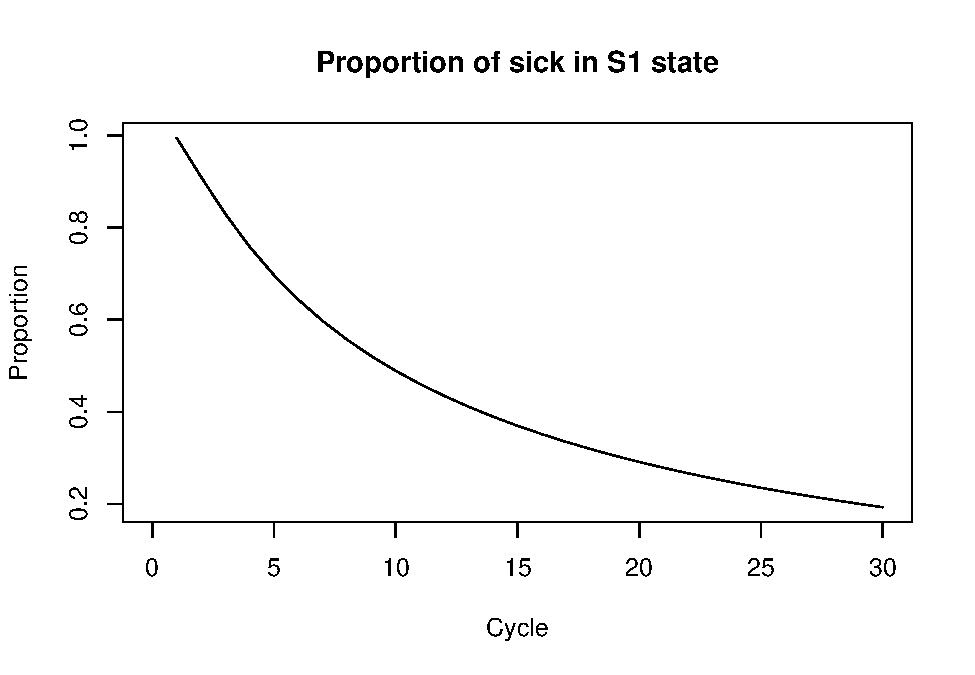
\includegraphics{VOI_toy_files/figure-latex/unnamed-chunk-13-1.pdf}

\hypertarget{enbs}{%
\section{10 ENBS}\label{enbs}}

\begin{Shaded}
\begin{Highlighting}[]
\CommentTok{# Population Values}
\CommentTok{# Discount rate}
\NormalTok{disc <-}\StringTok{ }\KeywordTok{c}\NormalTok{(}\FloatTok{0.03}\NormalTok{)}
\CommentTok{# Technology lifetime}
\NormalTok{LT   <-}\StringTok{ }\DecValTok{10}
\NormalTok{time <-}\StringTok{ }\KeywordTok{seq}\NormalTok{(}\DecValTok{0}\NormalTok{, LT)}
\CommentTok{# Per Annum Number of Individuals to Be Treated With Urate Lowering Therapy}
\CommentTok{# Present prevalence}
\NormalTok{prev <-}\StringTok{ }\FloatTok{0.010} \CommentTok{# In millions(1e6)}
\CommentTok{# Annual Incidence}
\NormalTok{incid <-}\StringTok{ }\DecValTok{147}\OperatorTok{*}\FloatTok{1e-6} \CommentTok{# In millions: 0.005*29.376e-3}
\CommentTok{# Total population afectd by technology calculated with `TotPop` function in Millions}
\NormalTok{tot_pop <-}\StringTok{ }\KeywordTok{TotPop}\NormalTok{(time,    }\CommentTok{# Function}
\NormalTok{                  prev, }
\NormalTok{                  incid, }
\NormalTok{                  disc) }

\CommentTok{# Population EVPSI}
\CommentTok{# Obervational study}
\NormalTok{pop_evsi_obs <-}\StringTok{ }\NormalTok{evsi_obs}
\NormalTok{pop_evsi_obs}\OperatorTok{$}\NormalTok{popEVSI <-}\StringTok{ }\NormalTok{pop_evsi_obs}\OperatorTok{$}\NormalTok{EVSI}\OperatorTok{*}\NormalTok{tot_pop}
\CommentTok{# RCT}
\NormalTok{pop_evsi_rct <-}\StringTok{ }\NormalTok{evsi_rct}
\NormalTok{pop_evsi_rct}\OperatorTok{$}\NormalTok{popEVSI <-}\StringTok{ }\NormalTok{pop_evsi_rct}\OperatorTok{$}\NormalTok{EVSI}\OperatorTok{*}\NormalTok{tot_pop}

\CommentTok{# Cost of research}
\CommentTok{# Obervational study}
\NormalTok{cost_res_obs <-}\StringTok{ }\KeywordTok{CostRes}\NormalTok{(}\DataTypeTok{fixed.cost =} \FloatTok{10000e-6}\NormalTok{,}
                        \DataTypeTok{samp.size =}\NormalTok{ n_obs,  }\CommentTok{# vector }
                        \DataTypeTok{cost.per.patient =} \FloatTok{500e-6}\NormalTok{, }\CommentTok{# In Million $}
                        \DataTypeTok{INMB =} \DecValTok{0}\NormalTok{,}
                        \DataTypeTok{clin.trial =} \OtherTok{FALSE}\NormalTok{)}
\CommentTok{# Data frame with cost of trial in Millions}
\NormalTok{cost_obs <-}\StringTok{ }\KeywordTok{data.frame}\NormalTok{(}\DataTypeTok{N =}\NormalTok{ n_obs, }\DataTypeTok{CS =}\NormalTok{ cost_res_obs)}
\CommentTok{# RCT}
\NormalTok{cost_res_rct <-}\StringTok{ }\KeywordTok{CostRes}\NormalTok{(}\DataTypeTok{fixed.cost =} \FloatTok{8000000e-6}\NormalTok{,}
                        \DataTypeTok{samp.size =}\NormalTok{ n_rct,  }\CommentTok{# vector }
                        \DataTypeTok{cost.per.patient =} \FloatTok{8500e-6}\NormalTok{, }\CommentTok{# In Million $}
                        \DataTypeTok{INMB =} \DecValTok{0}\NormalTok{,}
                        \DataTypeTok{clin.trial =} \OtherTok{TRUE}\NormalTok{) }
\CommentTok{# Data frame with cost of trial in Millions}
\NormalTok{cost_rct <-}\StringTok{ }\KeywordTok{data.frame}\NormalTok{(}\DataTypeTok{N =}\NormalTok{ n_rct, }\DataTypeTok{CS =}\NormalTok{ cost_res_rct)}

\CommentTok{# Create ENBS data frame}
\NormalTok{enbs_obs <-}\StringTok{ }\KeywordTok{merge}\NormalTok{(pop_evsi_obs, cost_obs, }\DataTypeTok{by =} \StringTok{"N"}\NormalTok{)}
\NormalTok{enbs_rct <-}\StringTok{ }\KeywordTok{merge}\NormalTok{(pop_evsi_rct, cost_rct, }\DataTypeTok{by =} \StringTok{"N"}\NormalTok{)}
\CommentTok{# Compute ENBS }
\NormalTok{enbs_obs}\OperatorTok{$}\NormalTok{ENBS <-}\StringTok{ }\NormalTok{enbs_obs}\OperatorTok{$}\NormalTok{popEVSI }\OperatorTok{-}\StringTok{ }\NormalTok{enbs_obs}\OperatorTok{$}\NormalTok{CS}
\NormalTok{enbs_rct}\OperatorTok{$}\NormalTok{ENBS <-}\StringTok{ }\NormalTok{enbs_rct}\OperatorTok{$}\NormalTok{popEVSI }\OperatorTok{-}\StringTok{ }\NormalTok{enbs_rct}\OperatorTok{$}\NormalTok{CS}
\CommentTok{# Compute OSS (n*)}
\NormalTok{enbs_obs}\OperatorTok{$}\NormalTok{nstar <-}\StringTok{ }\NormalTok{enbs_obs}\OperatorTok{$}\NormalTok{N[}\KeywordTok{which.max}\NormalTok{(enbs_obs}\OperatorTok{$}\NormalTok{ENBS)]}
\NormalTok{enbs_rct}\OperatorTok{$}\NormalTok{nstar <-}\StringTok{ }\NormalTok{enbs_rct}\OperatorTok{$}\NormalTok{N[}\KeywordTok{which.max}\NormalTok{(enbs_rct}\OperatorTok{$}\NormalTok{ENBS)]}
\CommentTok{# Append data frames}
\NormalTok{enbs_all <-}\StringTok{ }\KeywordTok{rbind}\NormalTok{(enbs_obs,}
\NormalTok{                  enbs_rct)}

\NormalTok{oss <-}\StringTok{ }\KeywordTok{summarise}\NormalTok{(}\KeywordTok{group_by}\NormalTok{(enbs_all, Study),}
                 \DataTypeTok{MaxENBS =} \KeywordTok{max}\NormalTok{(ENBS),}
                 \DataTypeTok{Nstar   =}\NormalTok{ N[}\KeywordTok{which.max}\NormalTok{(ENBS)])}
\end{Highlighting}
\end{Shaded}

\begin{verbatim}
## `summarise()` ungrouping output (override with `.groups` argument)
\end{verbatim}

\begin{Shaded}
\begin{Highlighting}[]
\CommentTok{# Plot ENBS, EVPSI and n*}
\CommentTok{# Create suitable data frames for plotting}
\NormalTok{enbs_obs_gg <-}\StringTok{ }\KeywordTok{melt}\NormalTok{(enbs_obs[, }\DecValTok{-3}\NormalTok{], }\DataTypeTok{id.vars =} \KeywordTok{c}\NormalTok{(}\StringTok{"Study"}\NormalTok{, }\StringTok{"N"}\NormalTok{, }\StringTok{"nstar"}\NormalTok{), }\DataTypeTok{value.name =} \StringTok{"Million"}\NormalTok{)}
\NormalTok{enbs_rct_gg <-}\StringTok{ }\KeywordTok{melt}\NormalTok{(enbs_rct[, }\DecValTok{-3}\NormalTok{], }\DataTypeTok{id.vars =} \KeywordTok{c}\NormalTok{(}\StringTok{"Study"}\NormalTok{, }\StringTok{"N"}\NormalTok{, }\StringTok{"nstar"}\NormalTok{), }\DataTypeTok{value.name =} \StringTok{"Million"}\NormalTok{)}
\CommentTok{# Append data frames for plotting}
\NormalTok{enbs_all_gg <-}\StringTok{ }\KeywordTok{rbind}\NormalTok{(enbs_obs_gg,}
\NormalTok{                     enbs_rct_gg)}
\KeywordTok{levels}\NormalTok{(enbs_all_gg}\OperatorTok{$}\NormalTok{Study) <-}\StringTok{ }\KeywordTok{c}\NormalTok{(}\KeywordTok{paste}\NormalTok{(}\StringTok{"Observational; n* = "}\NormalTok{, }\KeywordTok{comma}\NormalTok{(oss}\OperatorTok{$}\NormalTok{Nstar[}\DecValTok{1}\NormalTok{]), }\DataTypeTok{sep=}\StringTok{""}\NormalTok{), }
                               \KeywordTok{paste}\NormalTok{(}\StringTok{"RCT; n* = "}\NormalTok{, }\KeywordTok{comma}\NormalTok{(oss}\OperatorTok{$}\NormalTok{Nstar[}\DecValTok{2}\NormalTok{]), }\DataTypeTok{sep=}\StringTok{""}\NormalTok{))}

\KeywordTok{ggplot}\NormalTok{(enbs_all_gg, }\KeywordTok{aes}\NormalTok{(}\DataTypeTok{x =}\NormalTok{ N, }\DataTypeTok{y =}\NormalTok{ Million, }\DataTypeTok{colour =}\NormalTok{ variable, }\DataTypeTok{group =}\NormalTok{ variable)) }\OperatorTok{+}\StringTok{ }
\StringTok{  }\KeywordTok{facet_wrap}\NormalTok{(}\OperatorTok{~}\StringTok{ }\NormalTok{Study, }\DataTypeTok{scales =} \StringTok{"free_x"}\NormalTok{) }\OperatorTok{+}
\StringTok{  }\CommentTok{# geom_segment(data = oss, aes(x = Nstar, y = 0, xend = Nstar, yend = MaxENBS)) + }
\StringTok{  }\KeywordTok{geom_hline}\NormalTok{(}\KeywordTok{aes}\NormalTok{(}\DataTypeTok{yintercept=}\DecValTok{0}\NormalTok{), }\DataTypeTok{size =} \FloatTok{0.7}\NormalTok{, }\DataTypeTok{linetype =} \DecValTok{2}\NormalTok{, }\DataTypeTok{colour =} \StringTok{"gray"}\NormalTok{) }\OperatorTok{+}\StringTok{ }
\StringTok{  }\KeywordTok{geom_vline}\NormalTok{(}\KeywordTok{aes}\NormalTok{(}\DataTypeTok{xintercept =}\NormalTok{ nstar), }\DataTypeTok{size =} \FloatTok{0.7}\NormalTok{, }\DataTypeTok{linetype =} \DecValTok{2}\NormalTok{, }\DataTypeTok{colour =} \StringTok{"gray"}\NormalTok{) }\OperatorTok{+}\StringTok{ }
\StringTok{  }\KeywordTok{geom_point}\NormalTok{() }\OperatorTok{+}
\StringTok{  }\KeywordTok{geom_line}\NormalTok{() }\OperatorTok{+}
\StringTok{  }\KeywordTok{scale_x_continuous}\NormalTok{(}\DataTypeTok{breaks =} \KeywordTok{number_ticks}\NormalTok{(}\DecValTok{6}\NormalTok{), }\DataTypeTok{labels =}\NormalTok{ comma)}\OperatorTok{+}
\StringTok{  }\KeywordTok{scale_y_continuous}\NormalTok{(}\DataTypeTok{breaks =} \KeywordTok{number_ticks}\NormalTok{(}\DecValTok{6}\NormalTok{), }\DataTypeTok{labels =}\NormalTok{ comma, }\DataTypeTok{limits =} \KeywordTok{c}\NormalTok{(}\DecValTok{0}\NormalTok{, }\DecValTok{40}\NormalTok{))}\OperatorTok{+}
\StringTok{  }\KeywordTok{scale_colour_hue}\NormalTok{(}\StringTok{"Study design "}\NormalTok{, }\DataTypeTok{l=}\DecValTok{50}\NormalTok{,}
                   \DataTypeTok{labels=}\KeywordTok{c}\NormalTok{(}\StringTok{"popEVPSI(n) "}\NormalTok{, }\StringTok{"Cost of Research(n) "}\NormalTok{, }\StringTok{"ENBS(n) "}\NormalTok{)) }\OperatorTok{+}
\StringTok{  }\KeywordTok{xlab}\NormalTok{(}\StringTok{"Sample size (N)"}\NormalTok{) }\OperatorTok{+}
\StringTok{  }\KeywordTok{ylab}\NormalTok{(}\StringTok{"Value (Million $)"}\NormalTok{) }\OperatorTok{+}\StringTok{ }
\StringTok{  }\KeywordTok{theme_bw}\NormalTok{(}\DataTypeTok{base_size =} \DecValTok{14}\NormalTok{) }\OperatorTok{+}
\StringTok{  }\KeywordTok{theme}\NormalTok{(}\DataTypeTok{legend.position =} \StringTok{"bottom"}\NormalTok{,}
        \DataTypeTok{panel.spacing =} \KeywordTok{unit}\NormalTok{(}\DecValTok{2}\NormalTok{, }\StringTok{"lines"}\NormalTok{))}
\end{Highlighting}
\end{Shaded}

\begin{verbatim}
## Warning: Removed 3 rows containing missing values (geom_point).
\end{verbatim}

\begin{verbatim}
## Warning: Removed 1 row(s) containing missing values (geom_path).
\end{verbatim}

\includegraphics{VOI_toy_files/figure-latex/unnamed-chunk-14-1.pdf}

\end{document}
